\documentclass{article}

\setcounter{page}{1}
\setlength{\oddsidemargin}{0.in}
\setlength{\evensidemargin}{0.in}
\setlength{\textwidth}{6.5in}
\setlength{\topmargin}{-0.5in}
\setlength{\headheight}{0.17in}
\setlength{\headsep}{0.35in}
\setlength{\textheight}{9.in}
\setlength{\parindent}{0in}
\setlength{\parskip}{.1in}
\usepackage[T1]{fontenc}
\usepackage[round]{natbib}
\bibliographystyle{../../bst/sysbio}
\usepackage[fleqn]{amsmath}
\usepackage{amssymb}
\usepackage{xspace}
\usepackage{verbatim}
\usepackage{paralist}
\usepackage{setspace}
\usepackage{graphicx}
\usepackage{caption}
\usepackage{subcaption}
\usepackage{float}
\usepackage{url}
\usepackage{hyperref}
\hypersetup{backref, urlcolor=blue, linkcolor=blue, citecolor=blue,  colorlinks=true}

% use the fancyhdr package to allow both headers and footers
\usepackage{fancyhdr}
\pagestyle{fancy}
\fancyhf{} % clear all headers and footers
\fancyhead[RO,LE]{BEAST v1.7.5 Divergence-time Estimation Demo}
% \fancyhead[RO,LE]{2012}
\fancyfoot[LO,LE]{\footnotesize Tutorial content released under Creative Commons Attribution 3.0 Unported License.}
\fancyfoot[CE,CO]{}
\fancyfoot[RO,RE]{\thepage}
\renewcommand{\footrulewidth}{0.5pt}

% \floatstyle{boxed}
% \restylefloat{figure}
% \restylefloat{table}
\newfloat{textbox}{hptb}{lotb}
\floatname{textbox}{Box}

\newcommand{\execmd}[1]{\texttt{#1}\\}
\newcommand{\cmdopt}[1]{\texttt{#1}\xspace}
\newcommand{\cmd}[1]{\texttt{#1}\xspace}
\newcommand{\localfile}[1]{\textsf{#1}\xspace}
\newcommand{\QandA}[2]{\textit{#1}\footnote{#2}\xspace}
\newcommand{\todo}[1]{{\color{red}TODO: {#1}}\xspace}
\newcommand{\menutab}[1]{\textbf{\textit{#1}}\xspace}
\newcommand{\subItem}[2]{\menutab{#1}$\rightarrow$\menutab{#2}\xspace}
\newcommand{\subsubItem}[3]{\menutab{#1}$\rightarrow$\menutab{#2}$\rightarrow$\menutab{#3}\xspace}
\newcommand{\program}[1]{#1\xspace}
\newcommand{\plusbutton}{``$\boldsymbol{+}$''\xspace}
\newcommand{\beast}{\href{http://beast.bio.ed.ac.uk/Main_Page}{\program{BEAST}}\xspace}
\newcommand{\taxonset}[1]{{\bfseries\sffamily #1}\xspace}
\newcommand{\field}[1]{\texttt{#1}\xspace}
\newcommand{\fieldvalue}[1]{{\bfseries\sffamily #1}\xspace}
\newcommand{\questionfont}[1]{{\bfseries\sffamily\textit{#1}}\xspace}
\newcommand{\question}[1]{{\questionfont{#1}\\\vspace{2cm}}\xspace}


\begin{document}
{\Large\bf BEAST Divergence-time Lab}
{\singlespacing \tableofcontents}
\newpage
%###########################################################################################

\section{Objective}
The goal of this tutorial is to help you become familiar with using fossil data
to estimate time-calibrated phylogenetic trees in a Bayesian framework.
We will use an example dataset of DNA sequences of crocodylians (crocodiles and alligators)
and the software package \beast version 1.7.5.
We will work through the steps necessary for estimating the phylogenetic
relationships among crocodiles and alligators, while simultaneously using
fossil information and relaxed-clock models to calibrate the branches on the
tree to units of time (millions of years).

The stylistic conventions for this tutorial:

\begin{tabular}{|p{3.2in}|p{2.8in}|}
\hline	Names of files & \localfile{in this font}.\\
\hline	Web site URLs and other clickable links &  \href{http://www.google.com}{look like this}.\\
\hline	Nested menu items & \subsubItem{Top Name}{Mid Name}{Lowest}\\
\hline	\program{BEAUTi} menu tabs & \menutab{tab name}\\
\hline	\program{BEAUTi} option fields & \field{field name}\\
\hline	Field values that you enter & \fieldvalue{field value}\\
\hline	Questions for you to answer & \questionfont{look like this?}\\
\hline
\end{tabular}

% \section{Version and Author information}
% This tutorial was written for \beast version 1.7.5.

% This tutorial was written by Jamie Oaks.

\section{Background Information}

\section{The Data}

    \begin{figure}[htbp]
        \centering
        \fbox{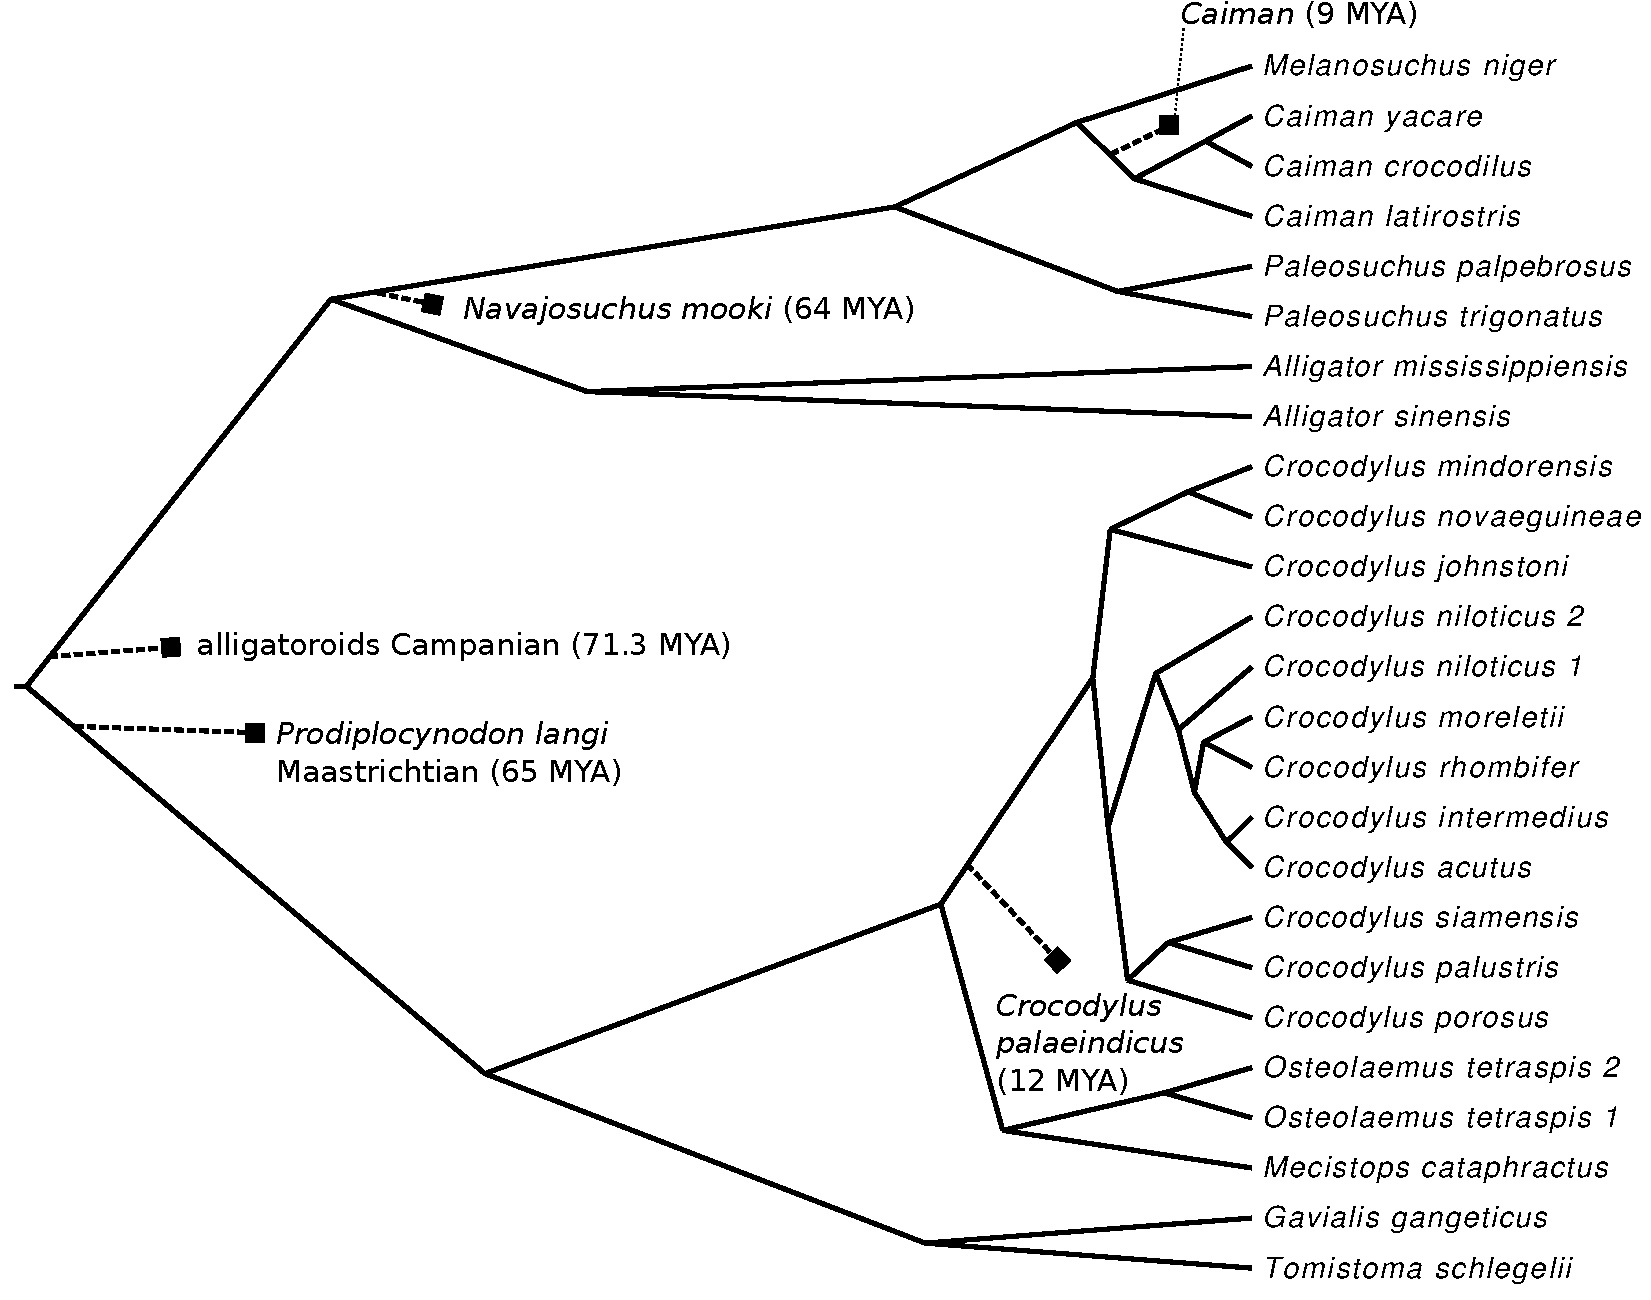
\includegraphics[width=0.8\textwidth]{../../images/crocodylia-fossils.pdf}}
        \caption{A phylogenetic estimate of Crocodylia with rough fossil placements.}
        \label{fig:crocFossils}
    \end{figure}

\section{Tutorial}
\newcounter{stepCounter}
\newcommand{\step}[2]{\addtocounter{stepCounter}{1} {\bf \hypertarget{step\arabic{stepCounter}}{Step \arabic{stepCounter}:}}\xspace #2\par}
\newcommand{\intermediate}[1]{#1}
\intermediate{\subsection{Downloads and Installations}}

\step{Download and install \beast.}{
    \beast is available at
    \href{http://beast.bio.ed.ac.uk/Main_Page}{\url{http://beast.bio.ed.ac.uk/Main_Page}}.
    This tutorial is written for version 1.7.5 of \beast.
}

\step{Download data files from \todo{HERE}.}{
    All of the files needed for this exercise can be downloaded from \todo{HERE}.
    \begin{textbox}
        \centering
        \fbox{\begin{minipage}[c][8em][c]{0.5\textwidth}
            \ttfamily
            \begin{compactitem}
                \item div-time-tutorial/
                \begin{compactitem}
                    \item crocodylia-cytb.nex
                    \item div-time-tutorial.pdf
                    \item yule.py
                    \item output/
                    \begin{compactitem}
                        \item crocodylia-cytb-run1.log
                    \end{compactitem}
                \end{compactitem}
            \end{compactitem}
        \end{minipage}}
        \caption{The files required for this tutorial.}
    \end{textbox}
}

\intermediate{\subsection{Setting up XML file with \program{BEAUTi}}}

\step{Launch BEAUTi.}{Begin by launching the \program{BEAUTi} program. If you
    are using Mac OSX or Windows, you should be able to do this by double
    clicking on the application. If everything is working correctly, a window
    should appear that looks something like Figure~\ref{fig:beautiInit}.
    \begin{figure}[htbp]
        \centering
        \fbox{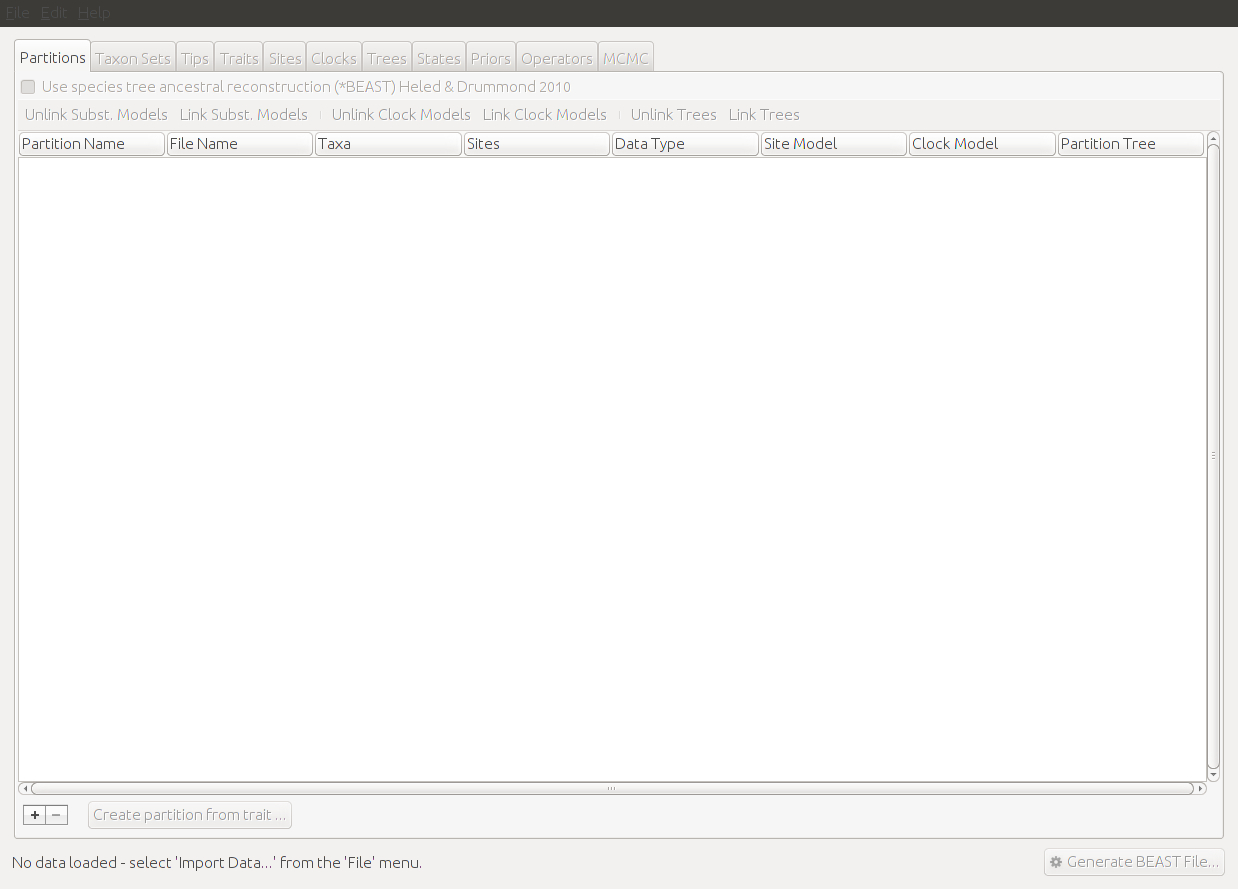
\includegraphics[width=0.7\textwidth]{../screenshots/beauti-init.jpg}}
        \caption{BEAUTi window.}
        \label{fig:beautiInit}
    \end{figure}
}

\step{Import the data in \localfile{crocodylia-cytb.nex}.}{
    Import the sequence data from the file \localfile{crocodylia-cytb.nex}
    using the drop-down menu \subItem{File}{Import Data} or using the
    \plusbutton button near the bottom-left corner of the window.

    You should be able to confirm that \program{BEAUTi} successfully imported
    24 sequences of nucleotides of length 1137
    (Figure~\ref{fig:beautiDataImported}).
    \begin{figure}[htbp]
        \centering
        \fbox{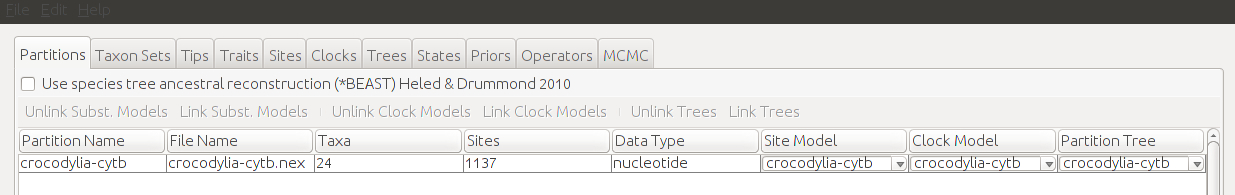
\includegraphics[width=0.8\textwidth]{../screenshots/beauti-data-imported.jpg}}
        \caption{The data successfully loaded by BEAUTi.}
        \label{fig:beautiDataImported}
    \end{figure}
}

\step{Inspect the alignment.}{
    Double click on the file name \localfile{crocodylia-cytb.nex} to bring up a
    window displaying the aligned sequences. It is always good practice to make
    sure everything looks as you expect. The cytochrome b gene is
    protein-coding, and aligns well across Crododylia without gaps.
}

\step{Define taxon sets.}{
    Next, we need to define some sets of taxa. Later, we will be able to use
    each of these sets to place priors on the age of their most recent common
    ancestor (MRCA).
    Let's start by defining the set for the clade
    containing the fossil taxon \emph{Navajosuchus mooki}; this clade has
    the family name Alligatoridae.

    Click on the \menutab{Taxon Sets} tab. Once in the \menutab{Taxon Sets}
    tab, click on the \plusbutton near the bottom-left corner of the window.
    This will create an untitled taxon set in the left-most box in the window.
    Change the name of this taxon set to \taxonset{Alligatoridae} and enter 65
    into Age column. This age is simply a starting value for the age of the
    MRCA of \taxonset{Alligatoridae}. It will ensure that the initial tree used
    to start the analysis is consistent with the lower bound of our fossil
    calibration (which will by 64 million years).
    
    We do not want to constrain \taxonset{Alligatoridae} to be monophyletic, so
    leave the \field{Mono?} box unchecked. Also, we are confident that
    \emph{Navajosuchus mooki} is nested within \taxonset{Alligatoridae}, and so
    we will leave the \field{Stem?} box unchecked. Because we only have a
    single tree, you can leave the \field{Tree} column unchanged.

    Next, we need to highlight the species that belong to
    \taxonset{Alligatoridae} within the \field{Excluded Taxa} window, and move
    them over to the \field{Included Taxa} window using the ``$\to$'' button.
    \taxonset{Alligatoridae} includes the following genera:
    \begin{compactitem}
        \item \emph{Alligator}
        \item \emph{Caiman}
        \item \emph{Melanosuchus}
        \item \emph{Paleosuchus}
    \end{compactitem}
    Highlight the species for these genera and move them over to the
    \field{Included Taxa} window.
    If you did everything correctly, your BEAUTi window should look like
    Figure~\ref{fig:beautiAlligatoridae}.
    \begin{figure}[htbp]
        \centering
        \fbox{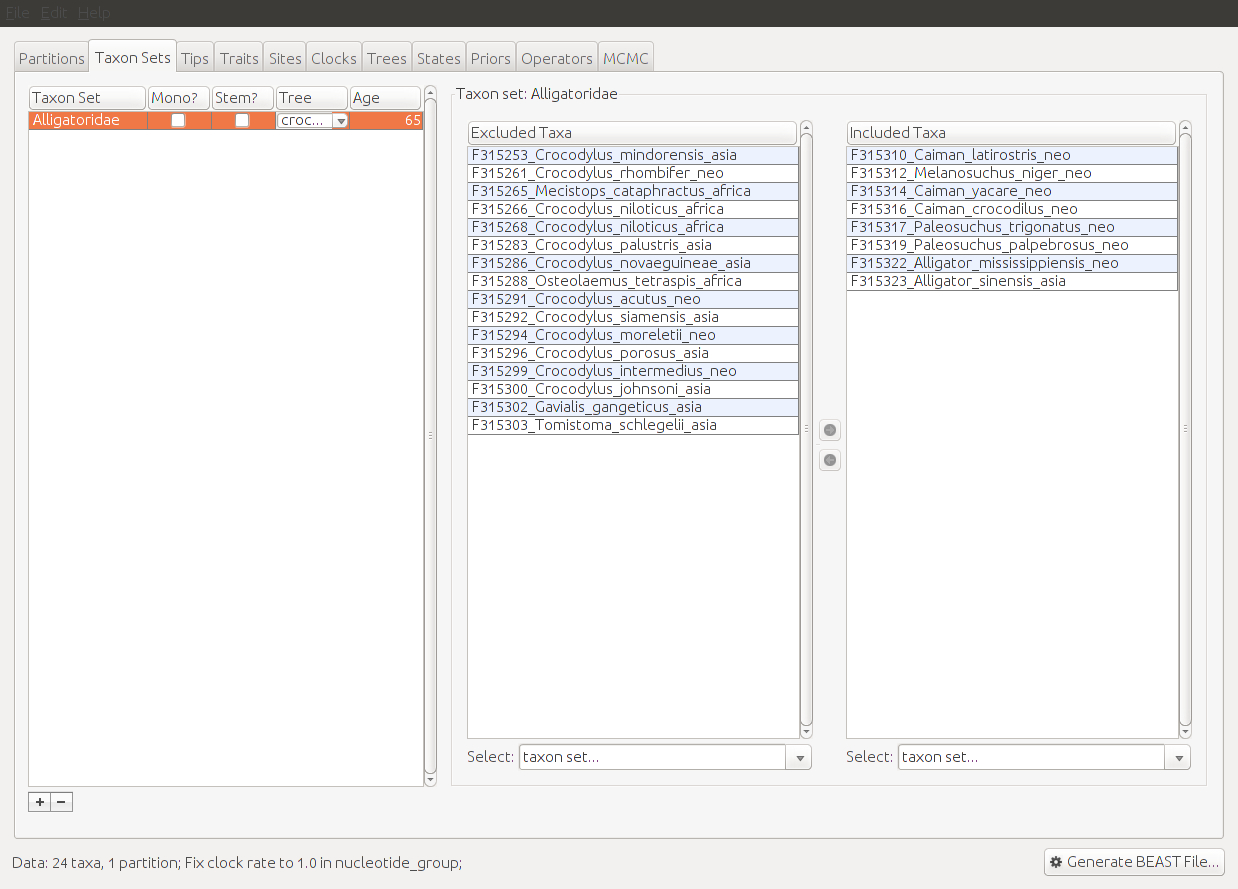
\includegraphics[width=0.9\textwidth]{../screenshots/beauti-taxon-set-alligatoridae.jpg}}
        \caption{The taxon set \taxonset{Alligatoridae} correctly defined.}
        \label{fig:beautiAlligatoridae}
    \end{figure}

    Next, let's define a taxon set for the genus \emph{Crocodylus}, which
    we will later use to specify an age prior corresponding to the fossil
    \emph{Crocodylus palaeindicus}. Click on the \plusbutton again to
    create a new taxon set, and name it \taxonset{Crocodylus}. Specify
    a starting age of 13, and leave the \field{Mono?} unchecked.

    We are confident that \emph{Crocodylus palaeindicus} is more closely
    related to all \emph{Crocodylus} species than to any other crocodylians.
    However, we are not confident that it is nested within extant species of
    \emph{Crocodylus} and suspect it is actually sister to them (as illustrated
    in Figure~\ref{fig:crocFossils}). As a result, we want to check the
    \field{Stem?} box. This specifies that the node we are interested in
    calibrating is the MRCA of all \emph{Crocodylus} sequences and their next
    closest relative (i.e., the stem node of \emph{Crocodylus}.
    Make sure the \taxonset{Crocodylus} taxon set is highlighted, and then
    highlight all the \emph{Crocodylus} species in the \field{Excluded Taxa}
    window and move them over to the \field{Included Taxa} window.

    Lastly, we need to define a taxon set for the genus \emph{Caiman}, which
    we will later use when specifying a calibration informed by the
    age of the oldest known \emph{Caiman} fossils.
    Click the \plusbutton to create a new taxon set, name it \taxonset{Caiman},
    specify a starting age of 10, and leave \field{Mono?} unchecked.
    As with \emph{Crocodylus} we don't know if the oldest \emph{Caiman} fossil
    taxa are nested within or sister to extant \emph{Caiman} species, and so
    we need to check the \field{Stem?} box.
    Highlight the three \emph{Caiman} species and move them over to the
    \field{Included Taxa} window.

    We will also be specifying a prior for the age of the root node of the
    tree, but we do not need to define a taxon set for this, because the root
    node is always defined by BEAUTi (you will see this later).

    Before you proceed to the next step, double check the three taxon sets
    you just defined and make sure you did not make a mistake with their
    ages or in selecting the species associated with them. Even a single
    misplaced species can lead to some very bizarre results!

    If you did everything correctly, your BEAUTi window should look similar to
    Figure~\ref{fig:beautiTaxSets}.

    \begin{figure}[htbp]
        \centering
        \fbox{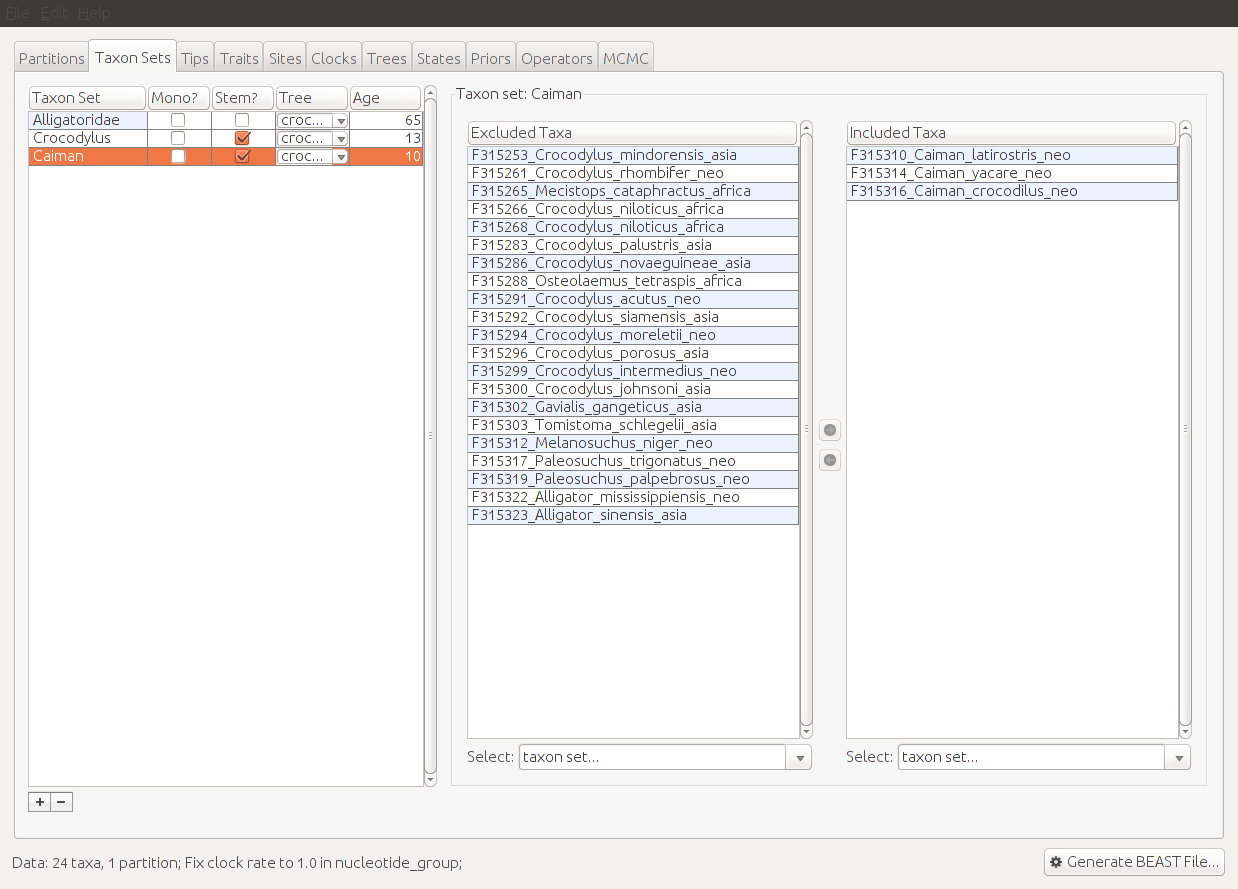
\includegraphics[width=0.9\textwidth]{../screenshots/beauti-taxon-sets.jpg}}
        \caption{All three taxon sets defined.}
        \label{fig:beautiTaxSets}
    \end{figure}
}

\step{Define geographic traits.}{
    Next we will use the \menutab{Traits} tab to define a new character for
    the geographic location of each species.
    This step is unrelated to divergence-time estimation. It will allow us to
    estimate the geographic locations of ancestral species across the
    phylogeny.
    Investigators are often interested in estimating ancestral states for
    characters of interest, so it is worth seeing how that can be done for in
    \beast while jointly estimating the phylogeny and divergence times.
    However, you will be learning all about ancestral character-state
    estimation in coming weeks, and so we will gloss over a lot of details to
    maintain the focus on divergence-time estimation.

    Once in the \menutab{Traits} tab, click the \plusbutton button (or the
    \field{Add trait} button). Once the \field{Create or Import Trait(s)}
    sub-window pops up, change the \field{Name} to \fieldvalue{geography}, set
    the \field{Type} to \fieldvalue{discrete}, and check the \field{Create a
    corresponding data partition} box
    (Figure~\ref{fig:beautiCreateTraitSubWindow}). Then, click \field{OK}.

    \begin{figure}[htbp]
        \centering
        \fbox{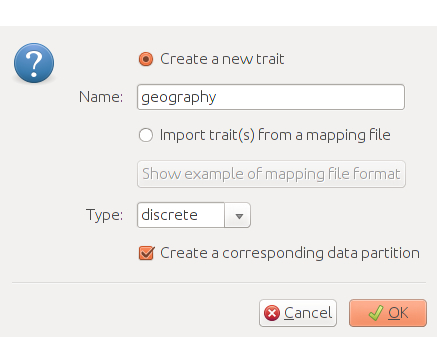
\includegraphics[width=0.4\textwidth]{../screenshots/beauti-create-trait-subwindow.jpg}}
        \caption{Creating a new trait.}
        \label{fig:beautiCreateTraitSubWindow}
    \end{figure}

    Next, click the \field{Guess trait values} button.  Once the sub-window
    pops up, select \field{Defined by its order} and set its drop-down field to
    \fieldvalue{last}. Put \fieldvalue{\_} (underscore) in the \field{with
    delimiter} field (Figure~\ref{fig:beautiGuessTraitSubWindow}). Click
    \field{OK}.
    If successful, the \menutab{Traits} tab should look like
    Figure~\ref{fig:beautiTraits}.

    \begin{figure}[htbp]
        \centering
        \fbox{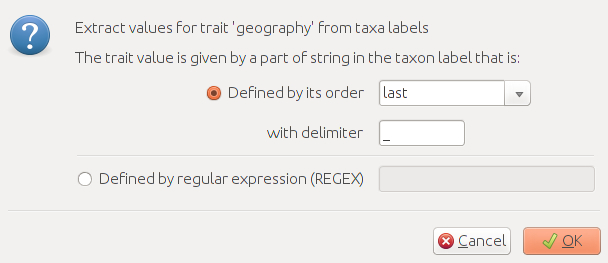
\includegraphics[width=0.5\textwidth]{../screenshots/beauti-guess-trait-subwindow.jpg}}
        \caption{\field{Guess trait} options.}
        \label{fig:beautiGuessTraitSubWindow}
    \end{figure}

    \begin{figure}[htbp]
        \centering
        \fbox{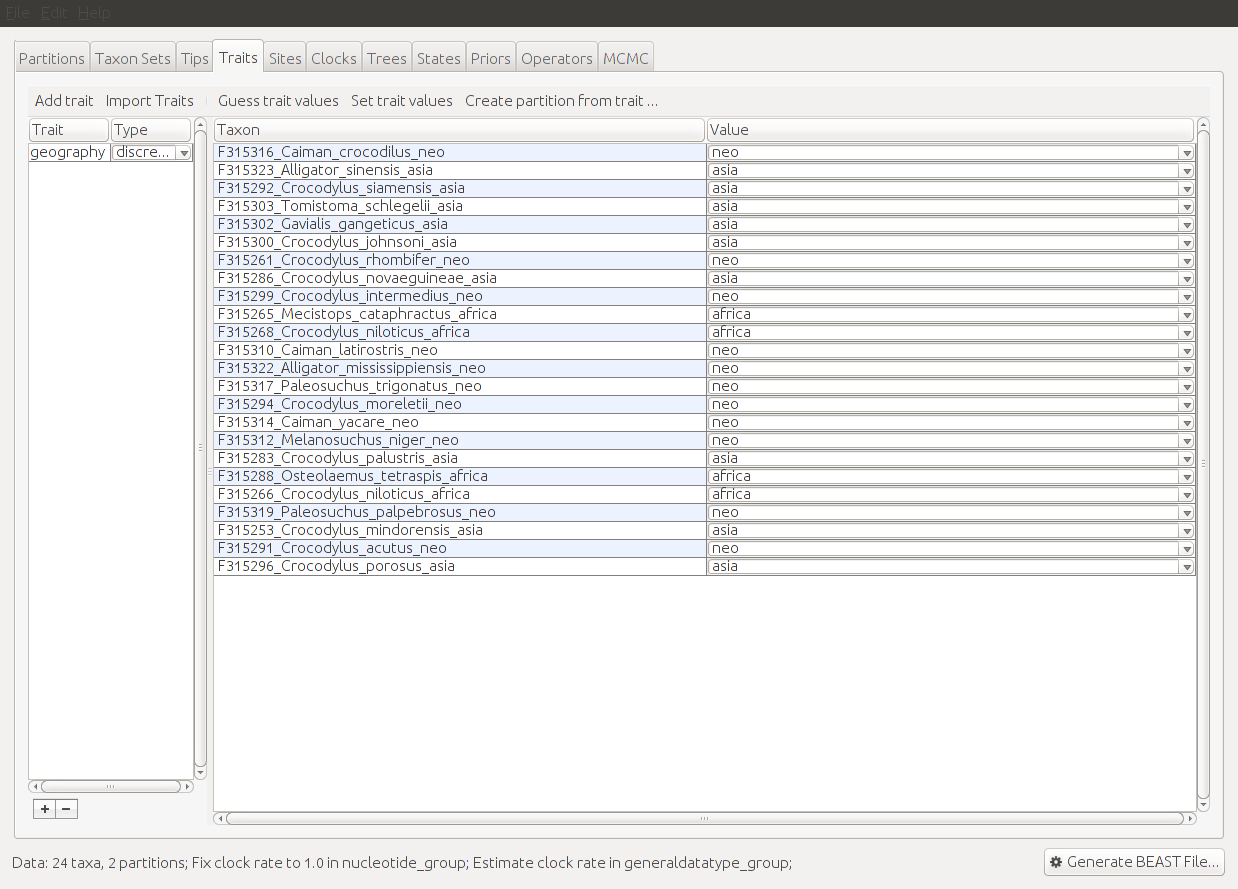
\includegraphics[width=0.8\textwidth]{../screenshots/beauti-traits.jpg}}
        \caption{Geographic traits successfully defined.}
        \label{fig:beautiTraits}
    \end{figure}
}

\step{Define Markov-chain models of substitution}{
    Next, we need to set up our continuous-time Markov chain (CTMC) models
    of substitution under the \menutab{Sites} tab.
    Once in the \menutab{Sites} tab, and with \fieldvalue{crocodylia-cytb} selected
    in the left \field{Substitution Model} window, select the following options:
    \begin{compactdesc}
        \centering
        \item[\field{Substitution Model:}] \fieldvalue{HKY}
        \item[\field{Base frequencies:}] \fieldvalue{Estimated}
        \item[\field{Site Heterogeneity Model:}] \fieldvalue{Gamma}
        \item[\field{Number of Gamma Categories:}] \fieldvalue{4}
        \item[\field{Partition into codon positions:}] \fieldvalue{3 partitions: positions 1, 2, 3}
    \end{compactdesc}
    Lastly, check all three \field{Unlink parameters} options (Figure~\ref{fig:beautiCytbModel}).

    \begin{figure}[htbp]
        \centering
        \fbox{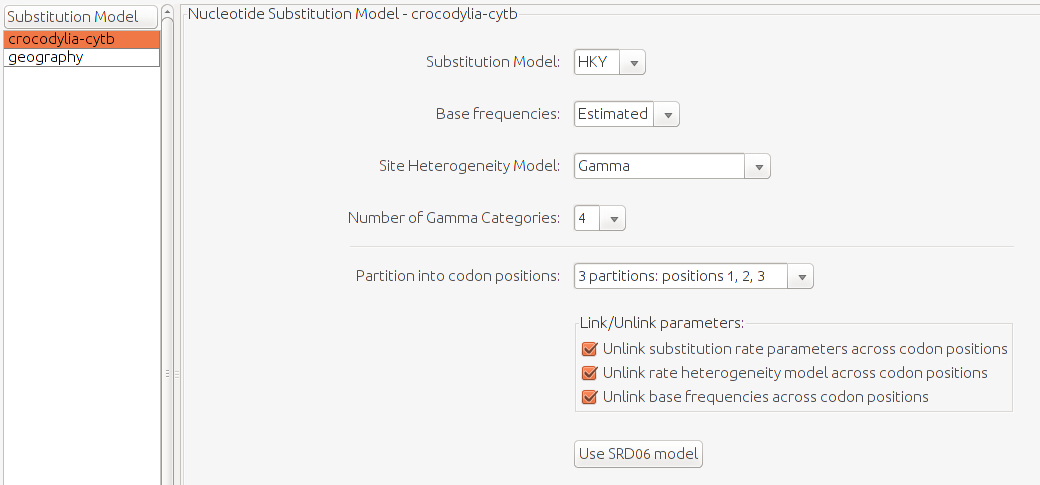
\includegraphics[width=0.8\textwidth]{../screenshots/beauti-cytb-model.jpg}}
        \caption{The CTMC model of nucleotide substitution for cytb.}
        \label{fig:beautiCytbModel}
    \end{figure}

    Next, select \fieldvalue{geography} in the left \field{Substitution Model}
    window, and select \fieldvalue{Asymmetric substitution model} for the
    \field{Discrete Trait Substitution Model} drop-down option. Check the box
    for \field{Infer social network with BSSVS} (Figure~\ref{fig:beautiGeoModel}).

    \begin{figure}[htbp]
        \centering
        \fbox{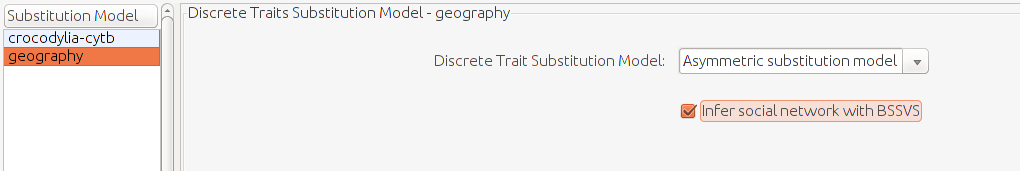
\includegraphics[width=0.8\textwidth]{../screenshots/beauti-geo-model.jpg}}
        \caption{The CTMC model for the geographic character.}
        \label{fig:beautiGeoModel}
    \end{figure}
}

\step{Define clock models.}{
    Next, we need to move to the \menutab{Clocks} tab and specify our models of
    branch rates across the tree. BEAUTi provides one strict-clock and
    three relaxed-clock options:
    \begin{compactdesc}
        \item[\fieldvalue{Strict clock}] Assumes a constant rate of
            substitution across all the branches of the tree.
        \item[\fieldvalue{Lognormal relaxed clock (Uncorrelated)}] Assumes that
            the rates of substitution on each branch of the tree are independent
            and drawn from a single, discretized lognormal distribution
            \citep{Drummond2006}.
        \item[\fieldvalue{Exponential relaxed clock (Uncorrelated)}]  Assumes that
            the rates of substitution on each branch of the tree are independent
            and drawn from a single, exponential distribution
            \citep{Drummond2006}.
        \item[\fieldvalue{Random local clock}] Uses Bayesian stochastic search
            variable selection (BSSVS) to average over local clock models
            (i.e., it averages over the number of rate changes and their
            locations) \citep{DrummondSuchard2010}.
    \end{compactdesc}

    In general, it is best to compare (or sample over) different clock models.
    But, for the sake of keeping this tutorial simple, we will select the most
    commonly used relaxed-clock model for the cytb data.
    For the \fieldvalue{crocodylia-cytb} data, select the \fieldvalue{Lognormal
    relaxed clock (Uncorrelated)}.
    For the \fieldvalue{geography} trait, select the \fieldvalue{Strict clock
    model}.
    Make sure to click the \field{Estimate} box for both models
    (Figure~\ref{fig:beautiClocks}).  You do not need to worry about the
    \field{Clock Model Group} options in the lower window.

    \begin{figure}[htbp]
        \centering
        \fbox{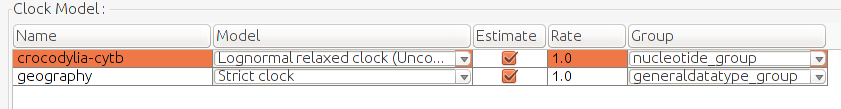
\includegraphics[width=0.8\textwidth]{../screenshots/beauti-clocks.jpg}}
        \caption{The clock-model settings.}
        \label{fig:beautiClocks}
    \end{figure}
}

\step{Select the tree prior.}{
    Next, let's move to the \menutab{Trees} tab to specify the prior and
    starting conditions for our tree.
    Select the \fieldvalue{Speciation: Birth-Death Process} option from the
    drop-down for the \field{Tree Prior} option.
    Select \fieldvalue{Random starting tree} in the lower window
    (Figure~\ref{fig:beautiTrees}.

    \begin{figure}[htbp]
        \centering
        \fbox{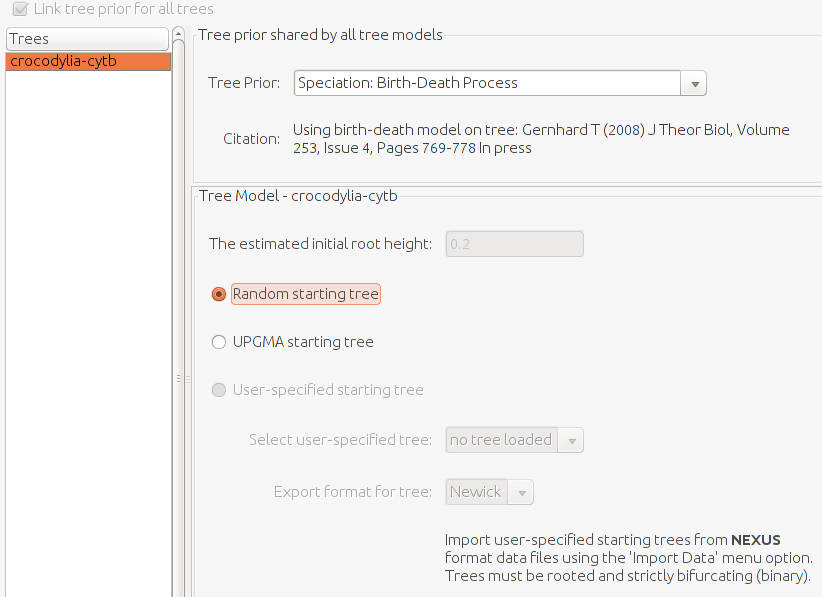
\includegraphics[width=0.8\textwidth]{../screenshots/beauti-trees.jpg}}
        \caption{The tree-prior settings.}
        \label{fig:beautiTrees}
    \end{figure}

    BEAUTi offers a number of tree prior options. Those labeled
    \fieldvalue{Speciation} are based on stochastic branching processes that
    assume the tips of the phylogeny are species. The \fieldvalue{Coalescent}
    tree priors are based on stochastic processes of lineage coalescence that
    assume the tips of the tree are gene copies within a population.
}

\step{Set the \field{States} options.}{
    Move to the \menutab{States} tab.
    With the \fieldvalue{crocodylia-cytb} \field{Partition} selected in the
    left column, leave all of the settings unchecked and the \field{Error
    Model} \fieldvalue{Off} (Figure~\ref{fig:beautiCytbStates}).
    Next, select the \fieldvalue{geography} \field{Partition} in the left column,
    check the \field{Reconstruct states at all ancestors} box, and leave all other
    options unchecked (Figure~\ref{fig:beautiGeoStates}).

    \begin{figure}[htbp]
        \centering
        \fbox{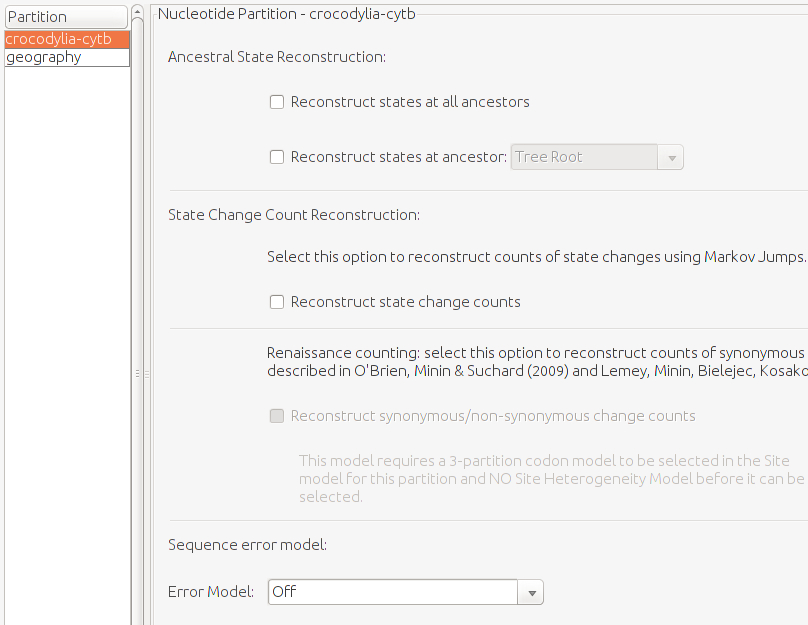
\includegraphics[width=0.7\textwidth]{../screenshots/beauti-cytb-states.jpg}}
        \caption{The \menutab{States} settings for cytb.}
        \label{fig:beautiCytbStates}
    \end{figure}
    \begin{figure}[htbp]
        \centering
        \fbox{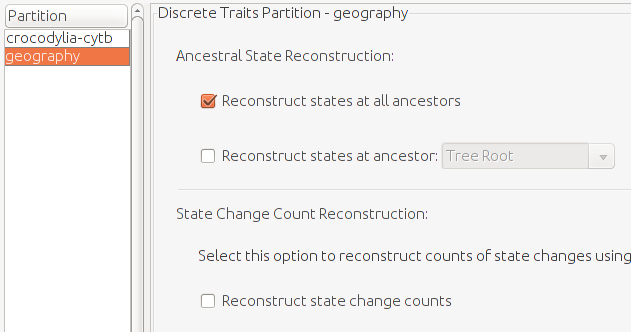
\includegraphics[width=0.5\textwidth]{../screenshots/beauti-geo-states.jpg}}
        \caption{The \menutab{States} settings for geography.}
        \label{fig:beautiGeoStates}
    \end{figure}
}

\step{Select priors for parameters.}{
    Move to the \menutab{Priors} tab.
    Here we see that all of the model parameters and statistics that we
    specified under the other tabs are listed.
    Now, we can specify prior probability distributions on the
    substitution-model parameters, relaxed-clock parameters, tree-prior
    parameters, and the time (age) of the most recent common ancestor (TMRCA)
    of the taxon sets we specified earlier.

    Let's start by selecting priors for the \fieldvalue{CP1.mu},
    \fieldvalue{CP2.mu}, and \fieldvalue{CP3.mu} parameters. These are
    relative-rate parameters that allow sites at the three codon positions to
    evolve at different rates. Based on our knowledge of the redundancy of the
    genetic code, we expect the sites at third-codon position to evolve more
    rapidly than the first and second codon sites \emph{a priori}.
    So we will specify our priors accordingly.

    Click on the \field{Prior} column for the \fieldvalue{CP1.mu} parameter.
    In the window that pops up, select an \fieldvalue{Exponential} \field{Prior
    Distribution}, and specify a \field{Mean} of \fieldvalue{0.5}.
    Do the same for \fieldvalue{CP2.mu}.
    For \fieldvalue{CP3.mu}, also select and \fieldvalue{Exponential}
    \field{Prior}, but set the \field{Mean} to \fieldvalue{5.0}
    (Figure~\ref{fig:beautiPriorsCPmu}).

    \begin{figure}[htbp]
        \centering
        \begin{subfigure}[b]{0.3\textwidth}
            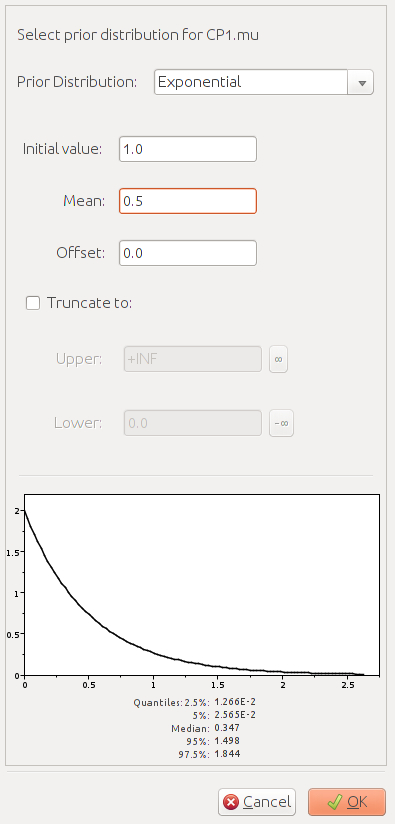
\includegraphics[width=\textwidth]{../screenshots/beauti-prior-cp1mu.jpg}
            \caption{CP1.mu.}
            \label{fig:beautiPriorsCP1mu}
        \end{subfigure}
        \begin{subfigure}[b]{0.3\textwidth}
            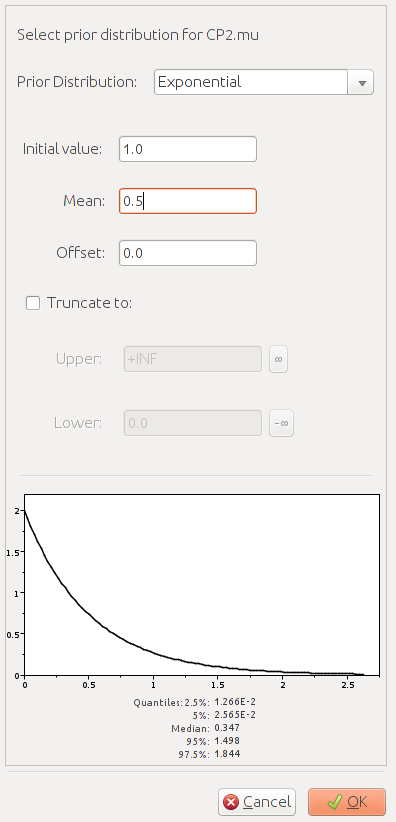
\includegraphics[width=\textwidth]{../screenshots/beauti-prior-cp2mu.jpg}
            \caption{CP2.mu.}
            \label{fig:beautiPriorsCP2mu}
        \end{subfigure}
        \begin{subfigure}[b]{0.3\textwidth}
            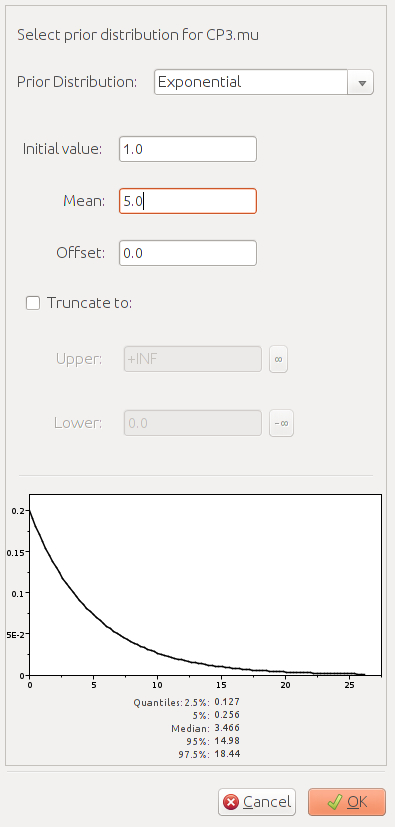
\includegraphics[width=\textwidth]{../screenshots/beauti-prior-cp3mu.jpg}
            \caption{CP2.mu.}
            \label{fig:beautiPriorsCP3mu}
        \end{subfigure}
        \caption{Priors for relative-rate parameters.}
        \label{fig:beautiPriorsCPmu}
    \end{figure}

    Next, click on the \field{Prior} column for the
    \fieldvalue{crocodylia-cytb.ucld.mean} parameter.
    This parameter controls the mean of the log-normal distribution from which
    the rates of each branch of the tree are drawn.
    Because we will be using fossils to calibrate the overall rate of substitution,
    we will use a very diffuse prior for this parameter.
    Select \fieldvalue{Exponential} for the \field{Prior}
    and specify \fieldvalue{0.05} for the \field{Mean}
    (Figure~\ref{fig:beautiPriorsUcldMean}).
    Because we will be specifying node-age priors in units of millions of
    years, the mean of 0.05 for prior on \fieldvalue{crocodylia-cytb.ucld.mean}
    translates to a mean rate of 5\% per million years.

    Specify an \fieldvalue{Exponential} prior for the
    \fieldvalue{geography.clock.rate}, but with a \field{Mean} of
    \fieldvalue{0.01} (Figure~\ref{fig:beautiPriorsClockRate}).

    The default prior for the \fieldvalue{birthDeath.meanGrowthRate}
    is \fieldvalue{Uniform} from \fieldvalue{0} to \fieldvalue{10000}.
    This is a very broad prior.
    Based on our knowledge of the crocodylian fossil record, we can get
    a rough idea of our prior expectations for this parameter.
    Given the age of the oldest crocodylian fossil is 71.3 million
    years, we know the height of our tree is at least that.
    Given that, we can calculate a pure-birth (Yule process) rate that has an
    expected tree height of 71.3 million years.
    I have included a Python script \localfile{yule.py} in the tutorial
    download that performs such calculations.

    \hspace{1cm}\cmd{Python yule.py height 71.3 24}

    which will produce the following output:

    \cmd{ntips = 24}\\
    \cmd{rate = 0.0389334947792}\\
    \cmd{height = 71.3}\\
    \cmd{length = 590.750974976}

    Thus, the largest we expect a pure-birth rate to be is around 0.04.
    This allows us to specify a much better prior than the default, while
    still diffuse.
    Specify an \fieldvalue{Exponential} prior for the
    \fieldvalue{birthDeath.meanGrowthRate}, but with a \field{Mean} of
    \fieldvalue{0.1} (Figure~\ref{fig:beautiPriorsBirthRate}).

    \begin{figure}[htbp]
        \centering
        \begin{subfigure}[b]{0.3\textwidth}
            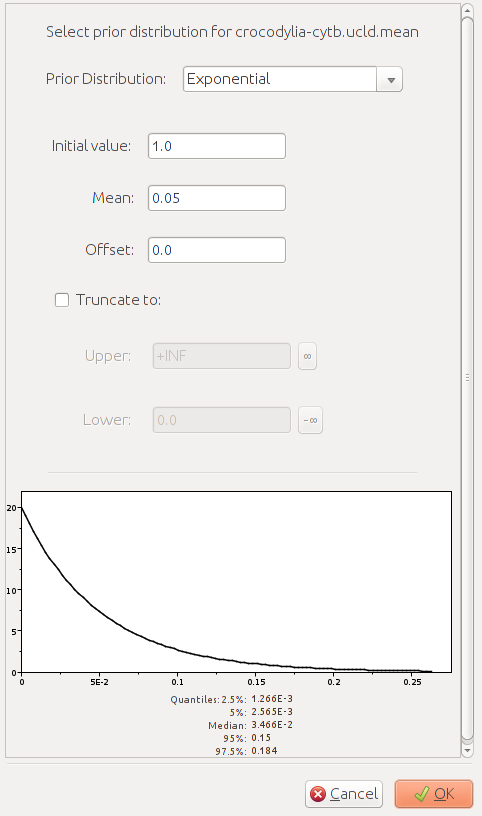
\includegraphics[width=\textwidth]{../screenshots/beauti-prior-ucldmean.jpg}
            \caption{crocodylia-cytb.ucld.mean.}
            \label{fig:beautiPriorsUcldMean}
        \end{subfigure}
        \begin{subfigure}[b]{0.29\textwidth}
            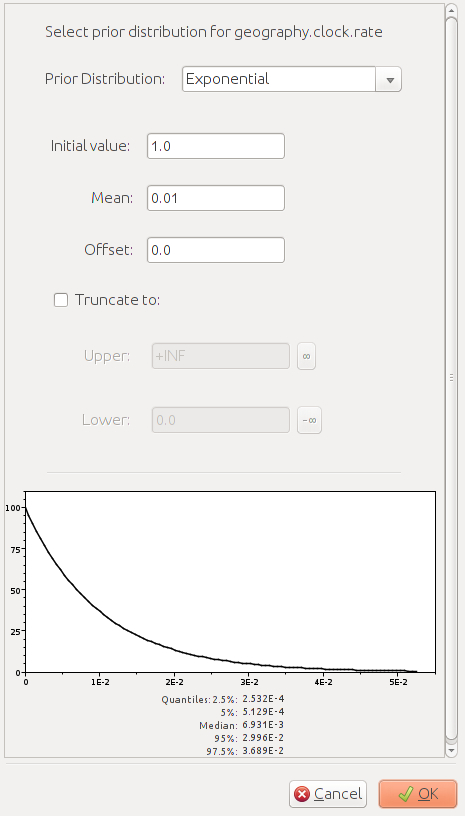
\includegraphics[width=\textwidth]{../screenshots/beauti-prior-clockrate.jpg}
            \caption{geography.clock.rate.}
            \label{fig:beautiPriorsClockRate}
        \end{subfigure}
        \begin{subfigure}[b]{0.31\textwidth}
            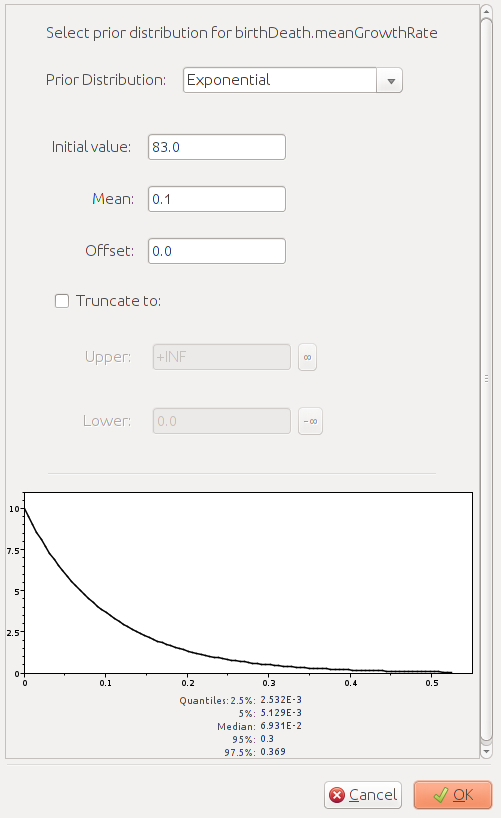
\includegraphics[width=\textwidth]{../screenshots/beauti-prior-birthrate.jpg}
            \caption{birthDeath.meanGrowthRate.}
            \label{fig:beautiPriorsBirthRate}
        \end{subfigure}
        \caption{Priors for clock rates and diversification rate.}
        \label{fig:beautiPriorsClocks}
    \end{figure}
}

\step{Select priors for node ages!}{
    Next, we need to specify our node-age priors based on fossil information.

    For \fieldvalue{tmrca(Alligatoridae)} select \fieldvalue{Gamma} for the
    \field{Prior Distribution}, and specify \fieldvalue{2} for both the
    \field{Shape} and \field{Scale} and \fieldvalue{64} for the
    \field{Offset}
    (Figure~\ref{fig:beautiPriorsAlligatoridae}).

    For \fieldvalue{tmrca(Crocodylus)} select \fieldvalue{Exponential} for the
    \field{Prior Distribution}, and specify \fieldvalue{10} for the mean
    and \fieldvalue{12} for the \field{Offset}
    (Figure~\ref{fig:beautiPriorsCrocodylus}).

    For \fieldvalue{tmrca(Caiman)} select \fieldvalue{Exponential} for the
    \field{Prior Distribution}, and specify \fieldvalue{4} for the mean
    and \fieldvalue{9} for the \field{Offset}
    (Figure~\ref{fig:beautiPriorsCaiman}).

    For \fieldvalue{treeModel.rootHeight} select \fieldvalue{Gamma} for the
    \field{Prior Distribution}, and specify \fieldvalue{78} for the
    \field{Initial value}, \fieldvalue{1.5} for the \field{Shape},
    \fieldvalue{6.0} for the \field{Scale}, and \fieldvalue{71.3} for the
    \field{Offset}. Also, make sure \field{Truncate to} is unchecked
    (Figure~\ref{fig:beautiPriorsRoot}).

    \begin{figure}[htbp]
        \centering
        \begin{subfigure}[b]{0.33\textwidth}
            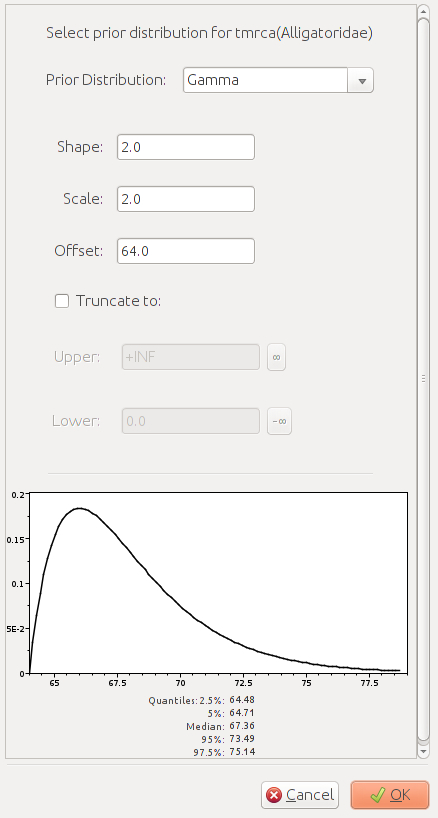
\includegraphics[width=\textwidth]{../screenshots/beauti-prior-alligatoridae.jpg}
            \caption{tmrca(Alligatoridae).}
            \label{fig:beautiPriorsAlligatoridae}
        \end{subfigure}
        \begin{subfigure}[b]{0.35\textwidth}
            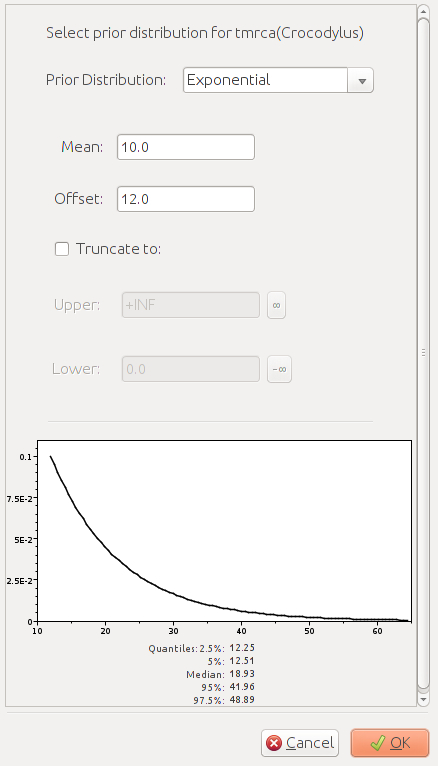
\includegraphics[width=\textwidth]{../screenshots/beauti-prior-crocodylus.jpg}
            \caption{tmrca(Crocodylus).}
            \label{fig:beautiPriorsCrocodylus}
        \end{subfigure}
        \begin{subfigure}[b]{0.35\textwidth}
            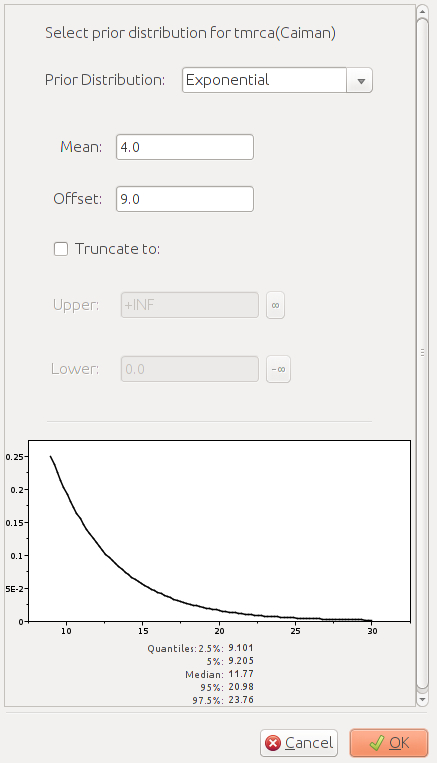
\includegraphics[width=\textwidth]{../screenshots/beauti-prior-caiman.jpg}
            \caption{tmrca(Caiman).}
            \label{fig:beautiPriorsCaiman}
        \end{subfigure}
        \begin{subfigure}[b]{0.315\textwidth}
            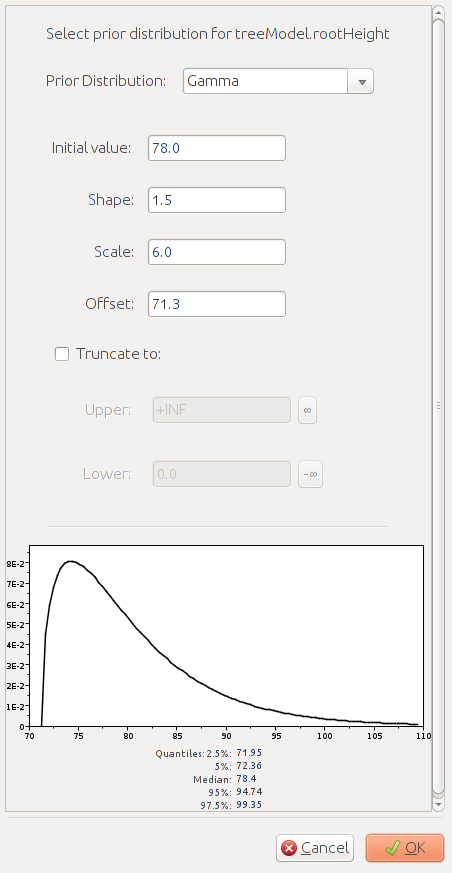
\includegraphics[width=\textwidth]{../screenshots/beauti-prior-root.jpg}
            \caption{treeModel.rootHeight.}
            \label{fig:beautiPriorsRoot}
        \end{subfigure}
        \caption{Priors for clock rates and diversification rate.}
        \label{fig:beautiPriorsClocks}
    \end{figure}
}


\newpage
\section{Quick version of the tutorial}
\setcounter{stepCounter}{0}
\renewcommand{\step}[2]{\addtocounter{stepCounter}{1} {\bf \hyperlink{step\arabic{stepCounter}}{Step \arabic{stepCounter}}:}\xspace #1\par}
\renewcommand{\intermediate}[1]{}
\intermediate{\subsection{Downloads and Installations}}

\step{Download and install \beast.}{
    \beast is available at
    \href{http://beast.bio.ed.ac.uk/Main_Page}{\url{http://beast.bio.ed.ac.uk/Main_Page}}.
    This tutorial is written for version 1.7.5 of \beast.
}

\step{Download data files from \todo{HERE}.}{
    All of the files needed for this exercise can be downloaded from \todo{HERE}.
    \begin{textbox}
        \centering
        \fbox{\begin{minipage}[c][8em][c]{0.5\textwidth}
            \ttfamily
            \begin{compactitem}
                \item div-time-tutorial/
                \begin{compactitem}
                    \item crocodylia-cytb.nex
                    \item div-time-tutorial.pdf
                    \item yule.py
                    \item output/
                    \begin{compactitem}
                        \item crocodylia-cytb-run1.log
                    \end{compactitem}
                \end{compactitem}
            \end{compactitem}
        \end{minipage}}
        \caption{The files required for this tutorial.}
    \end{textbox}
}

\intermediate{\subsection{Setting up XML file with \program{BEAUTi}}}

\step{Launch BEAUTi.}{Begin by launching the \program{BEAUTi} program. If you
    are using Mac OSX or Windows, you should be able to do this by double
    clicking on the application. If everything is working correctly, a window
    should appear that looks something like Figure~\ref{fig:beautiInit}.
    \begin{figure}[htbp]
        \centering
        \fbox{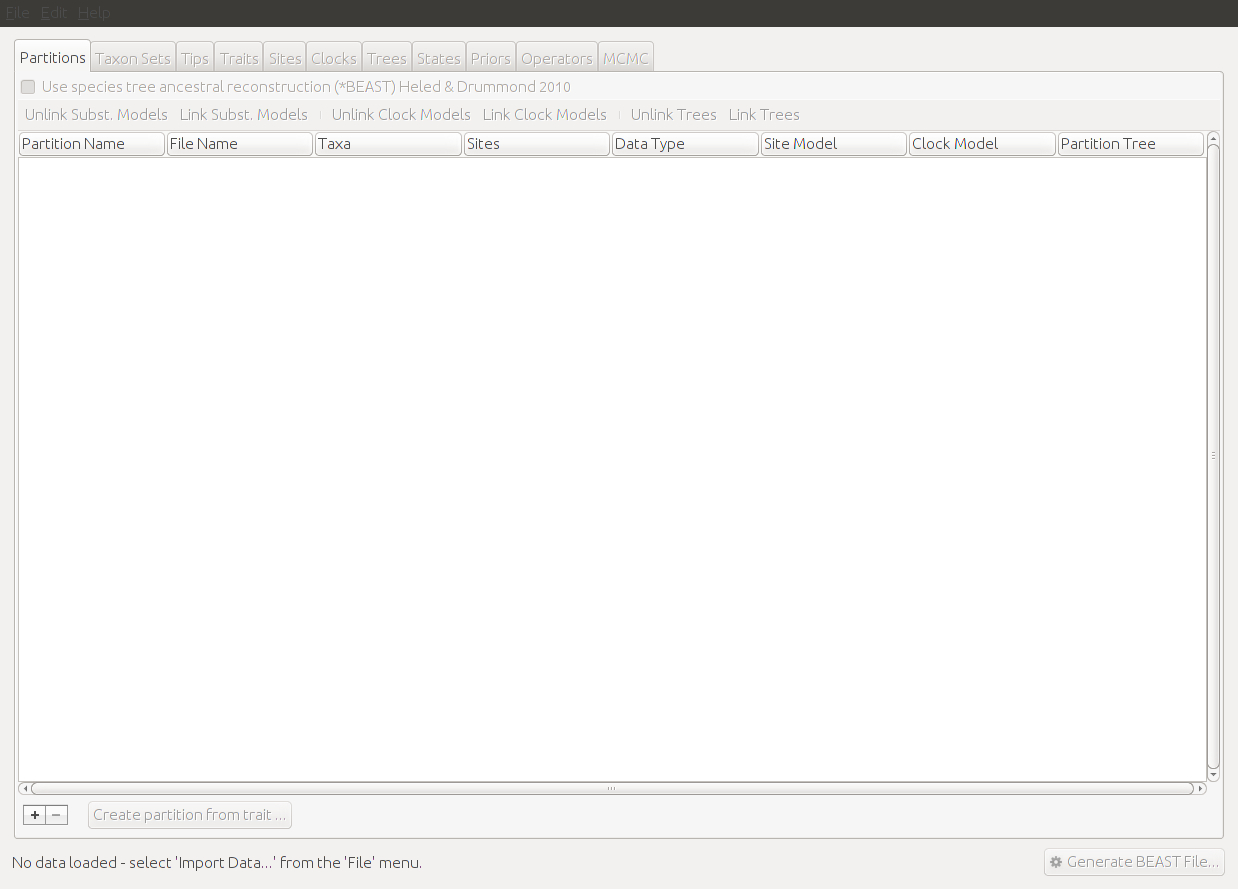
\includegraphics[width=0.7\textwidth]{../screenshots/beauti-init.jpg}}
        \caption{BEAUTi window.}
        \label{fig:beautiInit}
    \end{figure}
}

\step{Import the data in \localfile{crocodylia-cytb.nex}.}{
    Import the sequence data from the file \localfile{crocodylia-cytb.nex}
    using the drop-down menu \subItem{File}{Import Data} or using the
    \plusbutton button near the bottom-left corner of the window.

    You should be able to confirm that \program{BEAUTi} successfully imported
    24 sequences of nucleotides of length 1137
    (Figure~\ref{fig:beautiDataImported}).
    \begin{figure}[htbp]
        \centering
        \fbox{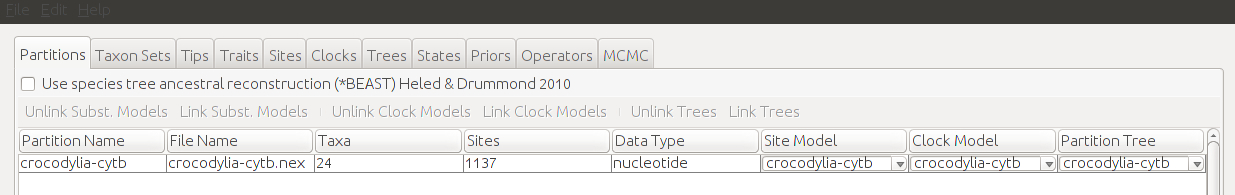
\includegraphics[width=0.8\textwidth]{../screenshots/beauti-data-imported.jpg}}
        \caption{The data successfully loaded by BEAUTi.}
        \label{fig:beautiDataImported}
    \end{figure}
}

\step{Inspect the alignment.}{
    Double click on the file name \localfile{crocodylia-cytb.nex} to bring up a
    window displaying the aligned sequences. It is always good practice to make
    sure everything looks as you expect. The cytochrome b gene is
    protein-coding, and aligns well across Crododylia without gaps.
}

\step{Define taxon sets.}{
    Next, we need to define some sets of taxa. Later, we will be able to use
    each of these sets to place priors on the age of their most recent common
    ancestor (MRCA).
    Let's start by defining the set for the clade
    containing the fossil taxon \emph{Navajosuchus mooki}; this clade has
    the family name Alligatoridae.

    Click on the \menutab{Taxon Sets} tab. Once in the \menutab{Taxon Sets}
    tab, click on the \plusbutton near the bottom-left corner of the window.
    This will create an untitled taxon set in the left-most box in the window.
    Change the name of this taxon set to \taxonset{Alligatoridae} and enter 65
    into Age column. This age is simply a starting value for the age of the
    MRCA of \taxonset{Alligatoridae}. It will ensure that the initial tree used
    to start the analysis is consistent with the lower bound of our fossil
    calibration (which will by 64 million years).
    
    We do not want to constrain \taxonset{Alligatoridae} to be monophyletic, so
    leave the \field{Mono?} box unchecked. Also, we are confident that
    \emph{Navajosuchus mooki} is nested within \taxonset{Alligatoridae}, and so
    we will leave the \field{Stem?} box unchecked. Because we only have a
    single tree, you can leave the \field{Tree} column unchanged.

    Next, we need to highlight the species that belong to
    \taxonset{Alligatoridae} within the \field{Excluded Taxa} window, and move
    them over to the \field{Included Taxa} window using the ``$\to$'' button.
    \taxonset{Alligatoridae} includes the following genera:
    \begin{compactitem}
        \item \emph{Alligator}
        \item \emph{Caiman}
        \item \emph{Melanosuchus}
        \item \emph{Paleosuchus}
    \end{compactitem}
    Highlight the species for these genera and move them over to the
    \field{Included Taxa} window.
    If you did everything correctly, your BEAUTi window should look like
    Figure~\ref{fig:beautiAlligatoridae}.
    \begin{figure}[htbp]
        \centering
        \fbox{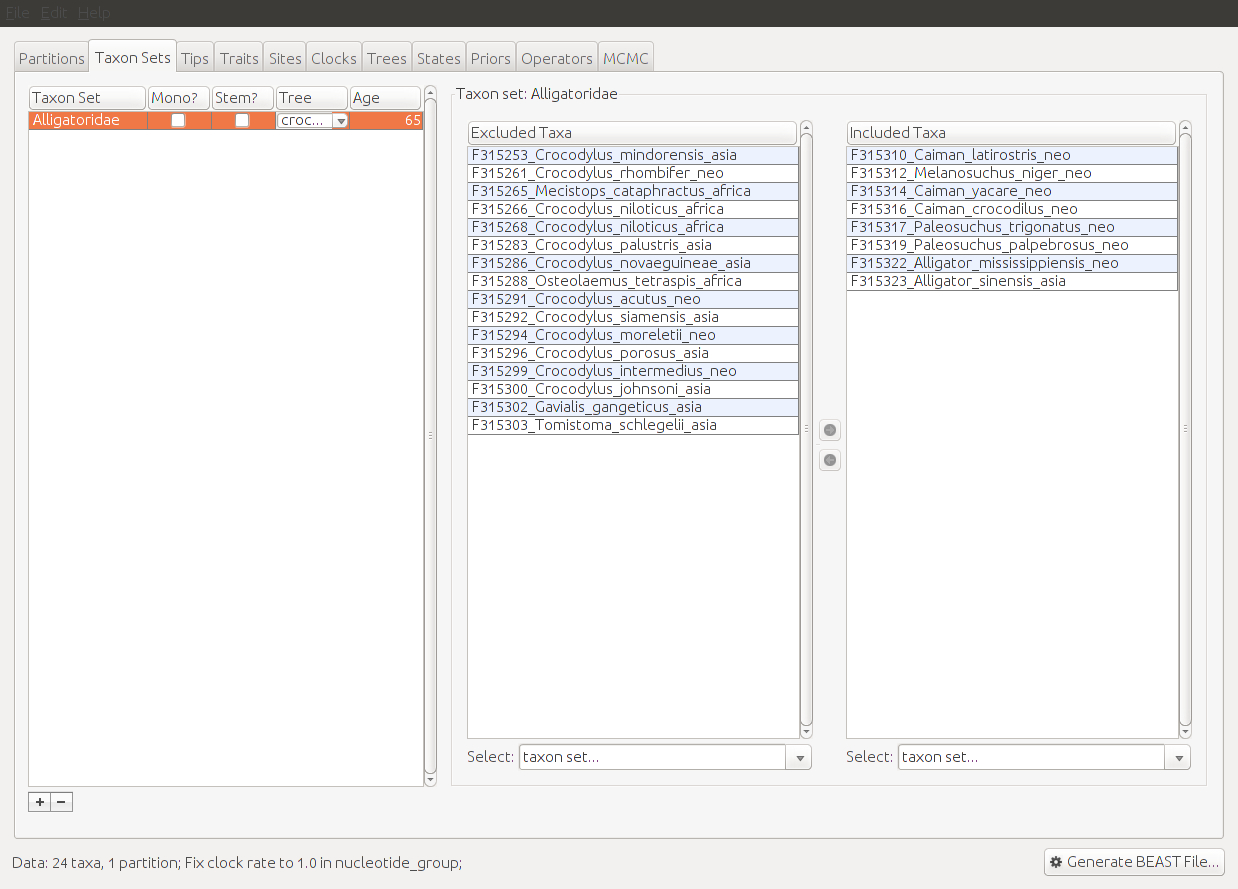
\includegraphics[width=0.9\textwidth]{../screenshots/beauti-taxon-set-alligatoridae.jpg}}
        \caption{The taxon set \taxonset{Alligatoridae} correctly defined.}
        \label{fig:beautiAlligatoridae}
    \end{figure}

    Next, let's define a taxon set for the genus \emph{Crocodylus}, which
    we will later use to specify an age prior corresponding to the fossil
    \emph{Crocodylus palaeindicus}. Click on the \plusbutton again to
    create a new taxon set, and name it \taxonset{Crocodylus}. Specify
    a starting age of 13, and leave the \field{Mono?} unchecked.

    We are confident that \emph{Crocodylus palaeindicus} is more closely
    related to all \emph{Crocodylus} species than to any other crocodylians.
    However, we are not confident that it is nested within extant species of
    \emph{Crocodylus} and suspect it is actually sister to them (as illustrated
    in Figure~\ref{fig:crocFossils}). As a result, we want to check the
    \field{Stem?} box. This specifies that the node we are interested in
    calibrating is the MRCA of all \emph{Crocodylus} sequences and their next
    closest relative (i.e., the stem node of \emph{Crocodylus}.
    Make sure the \taxonset{Crocodylus} taxon set is highlighted, and then
    highlight all the \emph{Crocodylus} species in the \field{Excluded Taxa}
    window and move them over to the \field{Included Taxa} window.

    Lastly, we need to define a taxon set for the genus \emph{Caiman}, which
    we will later use when specifying a calibration informed by the
    age of the oldest known \emph{Caiman} fossils.
    Click the \plusbutton to create a new taxon set, name it \taxonset{Caiman},
    specify a starting age of 10, and leave \field{Mono?} unchecked.
    As with \emph{Crocodylus} we don't know if the oldest \emph{Caiman} fossil
    taxa are nested within or sister to extant \emph{Caiman} species, and so
    we need to check the \field{Stem?} box.
    Highlight the three \emph{Caiman} species and move them over to the
    \field{Included Taxa} window.

    We will also be specifying a prior for the age of the root node of the
    tree, but we do not need to define a taxon set for this, because the root
    node is always defined by BEAUTi (you will see this later).

    Before you proceed to the next step, double check the three taxon sets
    you just defined and make sure you did not make a mistake with their
    ages or in selecting the species associated with them. Even a single
    misplaced species can lead to some very bizarre results!

    If you did everything correctly, your BEAUTi window should look similar to
    Figure~\ref{fig:beautiTaxSets}.

    \begin{figure}[htbp]
        \centering
        \fbox{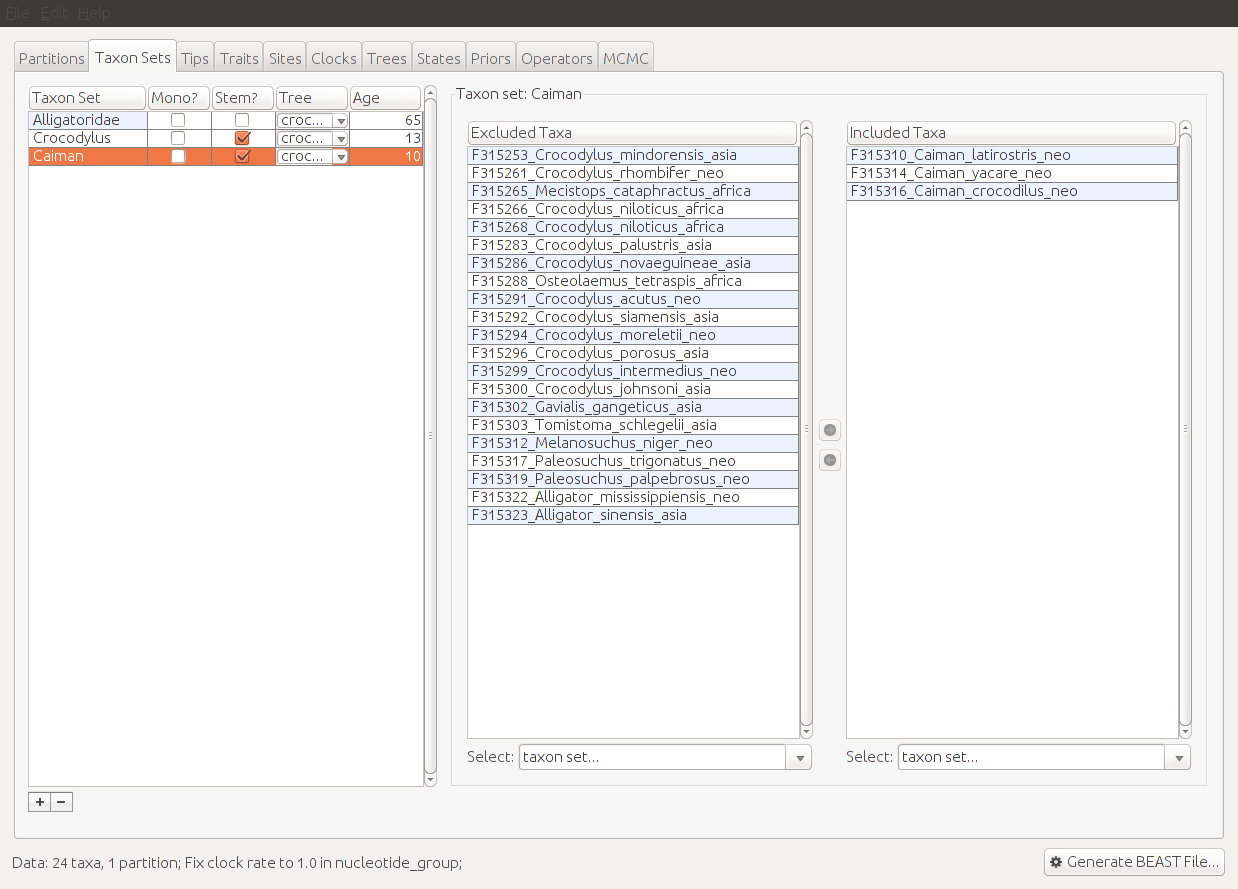
\includegraphics[width=0.9\textwidth]{../screenshots/beauti-taxon-sets.jpg}}
        \caption{All three taxon sets defined.}
        \label{fig:beautiTaxSets}
    \end{figure}
}

\step{Define geographic traits.}{
    Next we will use the \menutab{Traits} tab to define a new character for
    the geographic location of each species.
    This step is unrelated to divergence-time estimation. It will allow us to
    estimate the geographic locations of ancestral species across the
    phylogeny.
    Investigators are often interested in estimating ancestral states for
    characters of interest, so it is worth seeing how that can be done for in
    \beast while jointly estimating the phylogeny and divergence times.
    However, you will be learning all about ancestral character-state
    estimation in coming weeks, and so we will gloss over a lot of details to
    maintain the focus on divergence-time estimation.

    Once in the \menutab{Traits} tab, click the \plusbutton button (or the
    \field{Add trait} button). Once the \field{Create or Import Trait(s)}
    sub-window pops up, change the \field{Name} to \fieldvalue{geography}, set
    the \field{Type} to \fieldvalue{discrete}, and check the \field{Create a
    corresponding data partition} box
    (Figure~\ref{fig:beautiCreateTraitSubWindow}). Then, click \field{OK}.

    \begin{figure}[htbp]
        \centering
        \fbox{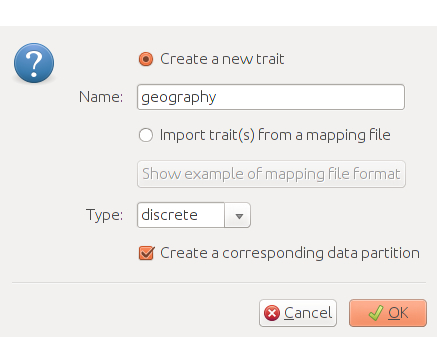
\includegraphics[width=0.4\textwidth]{../screenshots/beauti-create-trait-subwindow.jpg}}
        \caption{Creating a new trait.}
        \label{fig:beautiCreateTraitSubWindow}
    \end{figure}

    Next, click the \field{Guess trait values} button.  Once the sub-window
    pops up, select \field{Defined by its order} and set its drop-down field to
    \fieldvalue{last}. Put \fieldvalue{\_} (underscore) in the \field{with
    delimiter} field (Figure~\ref{fig:beautiGuessTraitSubWindow}). Click
    \field{OK}.
    If successful, the \menutab{Traits} tab should look like
    Figure~\ref{fig:beautiTraits}.

    \begin{figure}[htbp]
        \centering
        \fbox{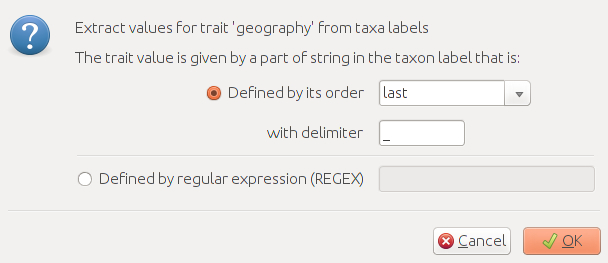
\includegraphics[width=0.5\textwidth]{../screenshots/beauti-guess-trait-subwindow.jpg}}
        \caption{\field{Guess trait} options.}
        \label{fig:beautiGuessTraitSubWindow}
    \end{figure}

    \begin{figure}[htbp]
        \centering
        \fbox{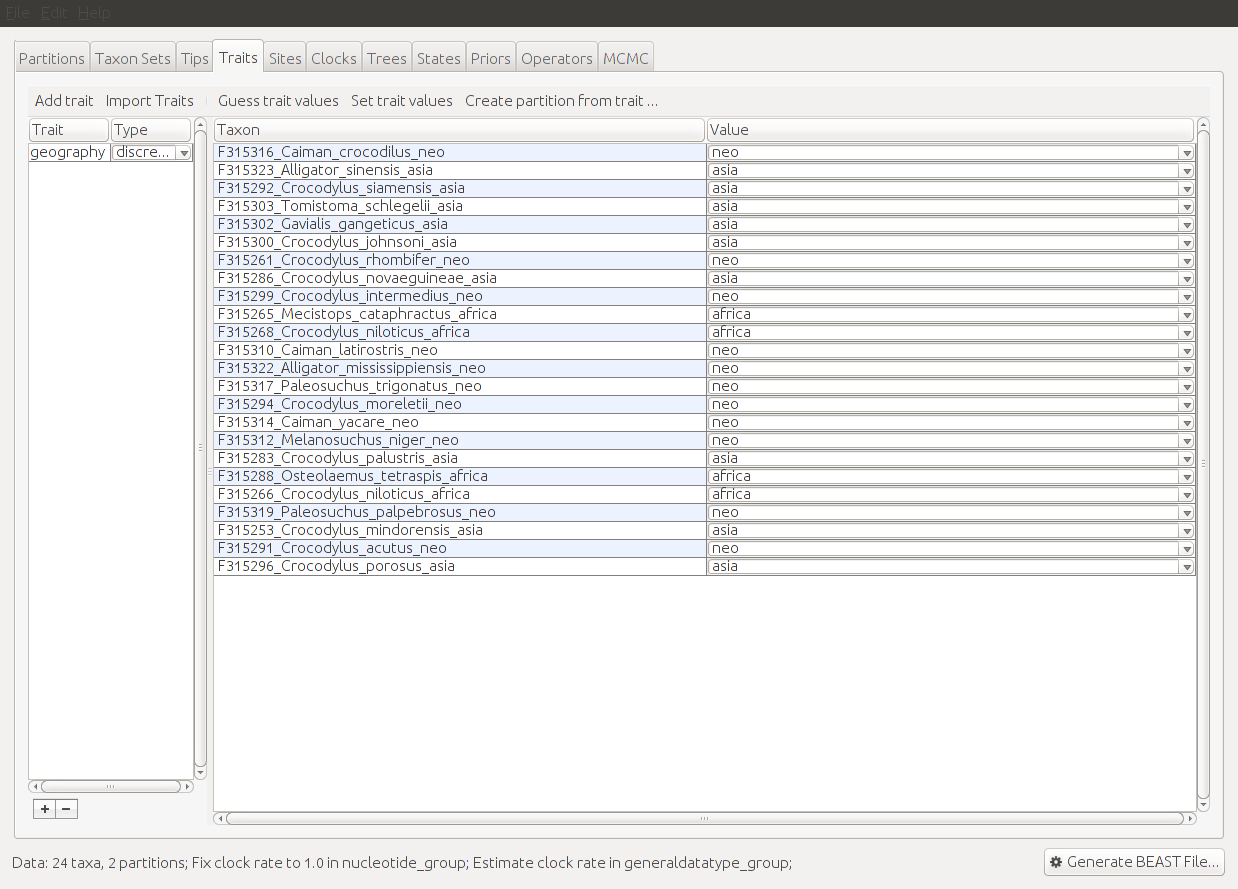
\includegraphics[width=0.8\textwidth]{../screenshots/beauti-traits.jpg}}
        \caption{Geographic traits successfully defined.}
        \label{fig:beautiTraits}
    \end{figure}
}

\step{Define Markov-chain models of substitution}{
    Next, we need to set up our continuous-time Markov chain (CTMC) models
    of substitution under the \menutab{Sites} tab.
    Once in the \menutab{Sites} tab, and with \fieldvalue{crocodylia-cytb} selected
    in the left \field{Substitution Model} window, select the following options:
    \begin{compactdesc}
        \centering
        \item[\field{Substitution Model:}] \fieldvalue{HKY}
        \item[\field{Base frequencies:}] \fieldvalue{Estimated}
        \item[\field{Site Heterogeneity Model:}] \fieldvalue{Gamma}
        \item[\field{Number of Gamma Categories:}] \fieldvalue{4}
        \item[\field{Partition into codon positions:}] \fieldvalue{3 partitions: positions 1, 2, 3}
    \end{compactdesc}
    Lastly, check all three \field{Unlink parameters} options (Figure~\ref{fig:beautiCytbModel}).

    \begin{figure}[htbp]
        \centering
        \fbox{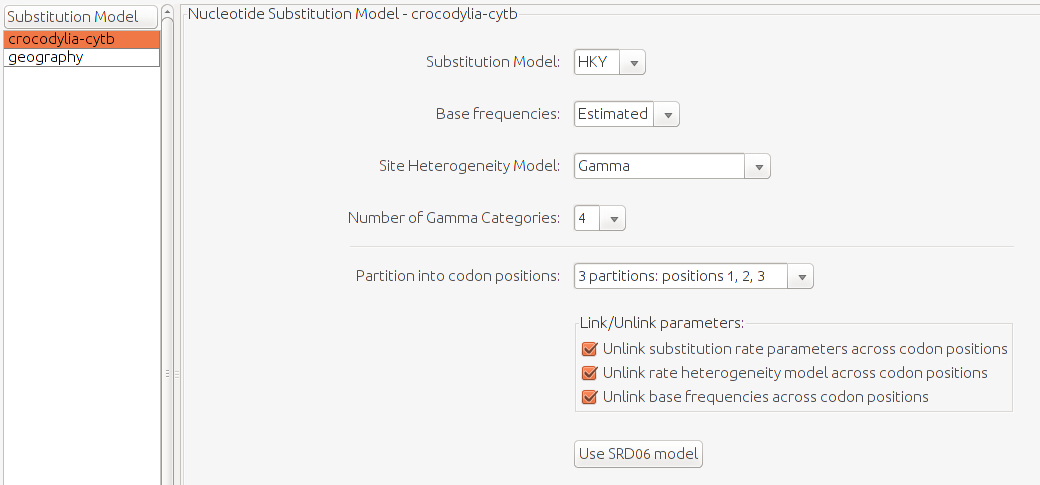
\includegraphics[width=0.8\textwidth]{../screenshots/beauti-cytb-model.jpg}}
        \caption{The CTMC model of nucleotide substitution for cytb.}
        \label{fig:beautiCytbModel}
    \end{figure}

    Next, select \fieldvalue{geography} in the left \field{Substitution Model}
    window, and select \fieldvalue{Asymmetric substitution model} for the
    \field{Discrete Trait Substitution Model} drop-down option. Check the box
    for \field{Infer social network with BSSVS} (Figure~\ref{fig:beautiGeoModel}).

    \begin{figure}[htbp]
        \centering
        \fbox{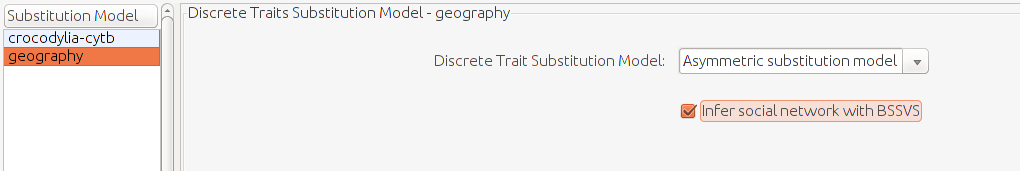
\includegraphics[width=0.8\textwidth]{../screenshots/beauti-geo-model.jpg}}
        \caption{The CTMC model for the geographic character.}
        \label{fig:beautiGeoModel}
    \end{figure}
}

\step{Define clock models.}{
    Next, we need to move to the \menutab{Clocks} tab and specify our models of
    branch rates across the tree. BEAUTi provides one strict-clock and
    three relaxed-clock options:
    \begin{compactdesc}
        \item[\fieldvalue{Strict clock}] Assumes a constant rate of
            substitution across all the branches of the tree.
        \item[\fieldvalue{Lognormal relaxed clock (Uncorrelated)}] Assumes that
            the rates of substitution on each branch of the tree are independent
            and drawn from a single, discretized lognormal distribution
            \citep{Drummond2006}.
        \item[\fieldvalue{Exponential relaxed clock (Uncorrelated)}]  Assumes that
            the rates of substitution on each branch of the tree are independent
            and drawn from a single, exponential distribution
            \citep{Drummond2006}.
        \item[\fieldvalue{Random local clock}] Uses Bayesian stochastic search
            variable selection (BSSVS) to average over local clock models
            (i.e., it averages over the number of rate changes and their
            locations) \citep{DrummondSuchard2010}.
    \end{compactdesc}

    In general, it is best to compare (or sample over) different clock models.
    But, for the sake of keeping this tutorial simple, we will select the most
    commonly used relaxed-clock model for the cytb data.
    For the \fieldvalue{crocodylia-cytb} data, select the \fieldvalue{Lognormal
    relaxed clock (Uncorrelated)}.
    For the \fieldvalue{geography} trait, select the \fieldvalue{Strict clock
    model}.
    Make sure to click the \field{Estimate} box for both models
    (Figure~\ref{fig:beautiClocks}).  You do not need to worry about the
    \field{Clock Model Group} options in the lower window.

    \begin{figure}[htbp]
        \centering
        \fbox{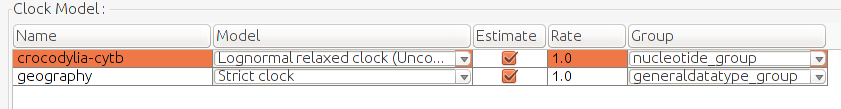
\includegraphics[width=0.8\textwidth]{../screenshots/beauti-clocks.jpg}}
        \caption{The clock-model settings.}
        \label{fig:beautiClocks}
    \end{figure}
}

\step{Select the tree prior.}{
    Next, let's move to the \menutab{Trees} tab to specify the prior and
    starting conditions for our tree.
    Select the \fieldvalue{Speciation: Birth-Death Process} option from the
    drop-down for the \field{Tree Prior} option.
    Select \fieldvalue{Random starting tree} in the lower window
    (Figure~\ref{fig:beautiTrees}.

    \begin{figure}[htbp]
        \centering
        \fbox{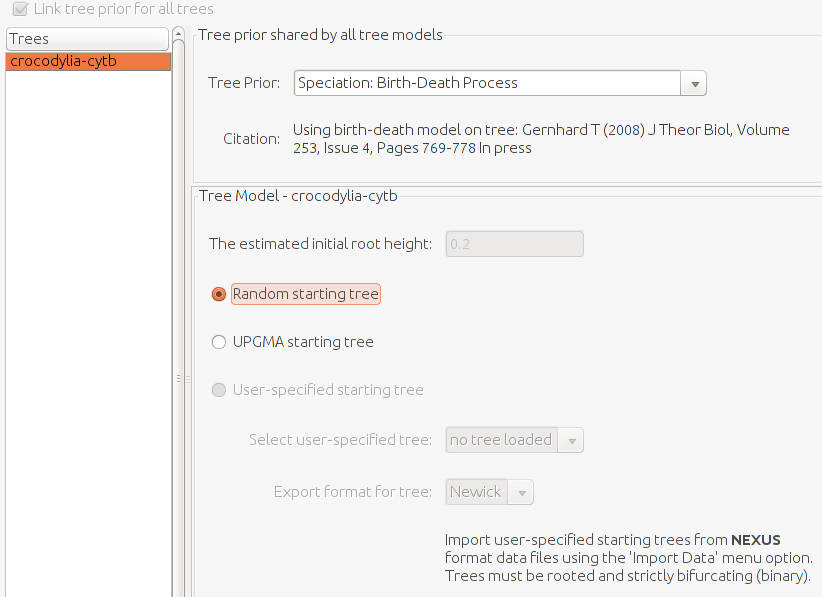
\includegraphics[width=0.8\textwidth]{../screenshots/beauti-trees.jpg}}
        \caption{The tree-prior settings.}
        \label{fig:beautiTrees}
    \end{figure}

    BEAUTi offers a number of tree prior options. Those labeled
    \fieldvalue{Speciation} are based on stochastic branching processes that
    assume the tips of the phylogeny are species. The \fieldvalue{Coalescent}
    tree priors are based on stochastic processes of lineage coalescence that
    assume the tips of the tree are gene copies within a population.
}

\step{Set the \field{States} options.}{
    Move to the \menutab{States} tab.
    With the \fieldvalue{crocodylia-cytb} \field{Partition} selected in the
    left column, leave all of the settings unchecked and the \field{Error
    Model} \fieldvalue{Off} (Figure~\ref{fig:beautiCytbStates}).
    Next, select the \fieldvalue{geography} \field{Partition} in the left column,
    check the \field{Reconstruct states at all ancestors} box, and leave all other
    options unchecked (Figure~\ref{fig:beautiGeoStates}).

    \begin{figure}[htbp]
        \centering
        \fbox{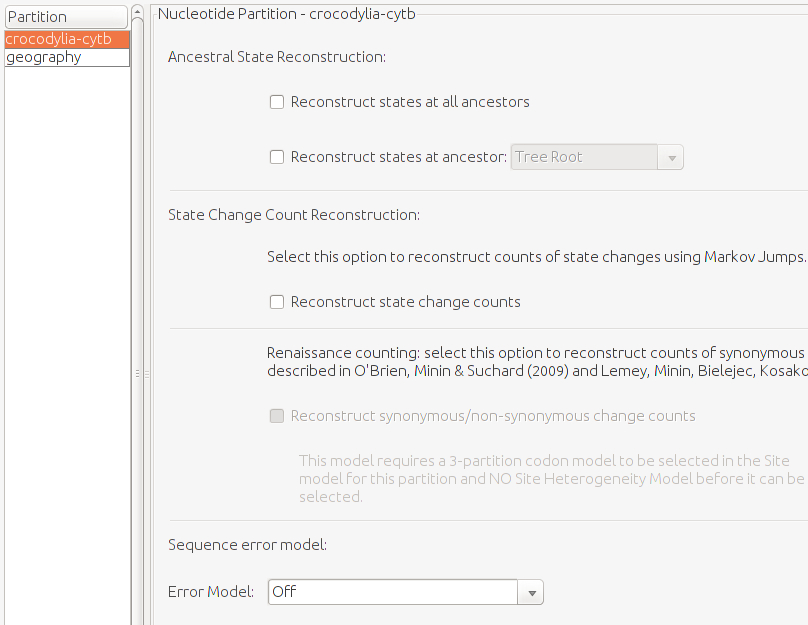
\includegraphics[width=0.7\textwidth]{../screenshots/beauti-cytb-states.jpg}}
        \caption{The \menutab{States} settings for cytb.}
        \label{fig:beautiCytbStates}
    \end{figure}
    \begin{figure}[htbp]
        \centering
        \fbox{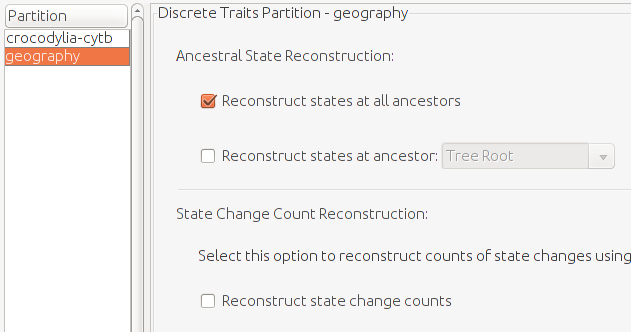
\includegraphics[width=0.5\textwidth]{../screenshots/beauti-geo-states.jpg}}
        \caption{The \menutab{States} settings for geography.}
        \label{fig:beautiGeoStates}
    \end{figure}
}

\step{Select priors for parameters.}{
    Move to the \menutab{Priors} tab.
    Here we see that all of the model parameters and statistics that we
    specified under the other tabs are listed.
    Now, we can specify prior probability distributions on the
    substitution-model parameters, relaxed-clock parameters, tree-prior
    parameters, and the time (age) of the most recent common ancestor (TMRCA)
    of the taxon sets we specified earlier.

    Let's start by selecting priors for the \fieldvalue{CP1.mu},
    \fieldvalue{CP2.mu}, and \fieldvalue{CP3.mu} parameters. These are
    relative-rate parameters that allow sites at the three codon positions to
    evolve at different rates. Based on our knowledge of the redundancy of the
    genetic code, we expect the sites at third-codon position to evolve more
    rapidly than the first and second codon sites \emph{a priori}.
    So we will specify our priors accordingly.

    Click on the \field{Prior} column for the \fieldvalue{CP1.mu} parameter.
    In the window that pops up, select an \fieldvalue{Exponential} \field{Prior
    Distribution}, and specify a \field{Mean} of \fieldvalue{0.5}.
    Do the same for \fieldvalue{CP2.mu}.
    For \fieldvalue{CP3.mu}, also select and \fieldvalue{Exponential}
    \field{Prior}, but set the \field{Mean} to \fieldvalue{5.0}
    (Figure~\ref{fig:beautiPriorsCPmu}).

    \begin{figure}[htbp]
        \centering
        \begin{subfigure}[b]{0.3\textwidth}
            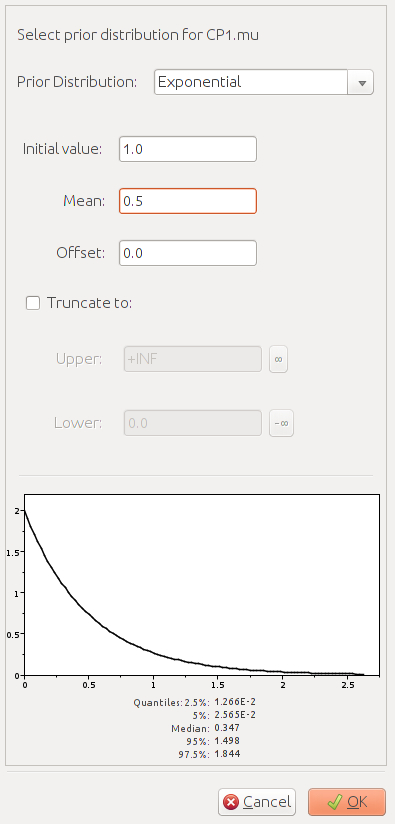
\includegraphics[width=\textwidth]{../screenshots/beauti-prior-cp1mu.jpg}
            \caption{CP1.mu.}
            \label{fig:beautiPriorsCP1mu}
        \end{subfigure}
        \begin{subfigure}[b]{0.3\textwidth}
            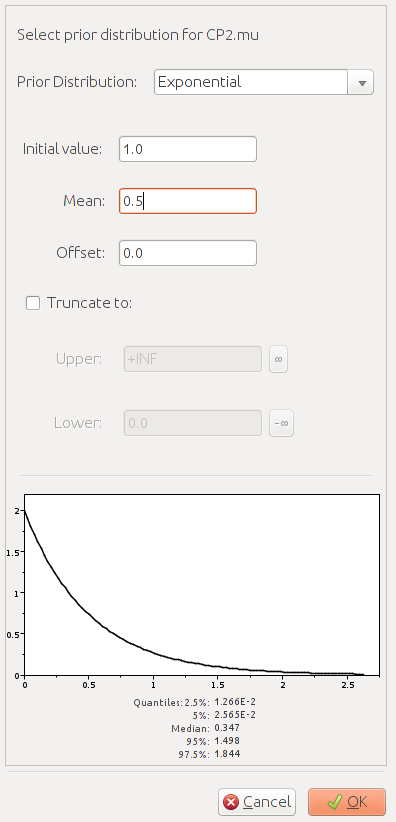
\includegraphics[width=\textwidth]{../screenshots/beauti-prior-cp2mu.jpg}
            \caption{CP2.mu.}
            \label{fig:beautiPriorsCP2mu}
        \end{subfigure}
        \begin{subfigure}[b]{0.3\textwidth}
            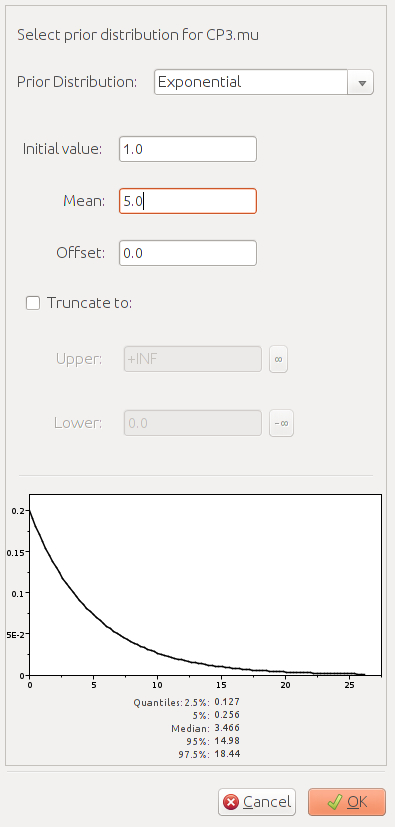
\includegraphics[width=\textwidth]{../screenshots/beauti-prior-cp3mu.jpg}
            \caption{CP2.mu.}
            \label{fig:beautiPriorsCP3mu}
        \end{subfigure}
        \caption{Priors for relative-rate parameters.}
        \label{fig:beautiPriorsCPmu}
    \end{figure}

    Next, click on the \field{Prior} column for the
    \fieldvalue{crocodylia-cytb.ucld.mean} parameter.
    This parameter controls the mean of the log-normal distribution from which
    the rates of each branch of the tree are drawn.
    Because we will be using fossils to calibrate the overall rate of substitution,
    we will use a very diffuse prior for this parameter.
    Select \fieldvalue{Exponential} for the \field{Prior}
    and specify \fieldvalue{0.05} for the \field{Mean}
    (Figure~\ref{fig:beautiPriorsUcldMean}).
    Because we will be specifying node-age priors in units of millions of
    years, the mean of 0.05 for prior on \fieldvalue{crocodylia-cytb.ucld.mean}
    translates to a mean rate of 5\% per million years.

    Specify an \fieldvalue{Exponential} prior for the
    \fieldvalue{geography.clock.rate}, but with a \field{Mean} of
    \fieldvalue{0.01} (Figure~\ref{fig:beautiPriorsClockRate}).

    The default prior for the \fieldvalue{birthDeath.meanGrowthRate}
    is \fieldvalue{Uniform} from \fieldvalue{0} to \fieldvalue{10000}.
    This is a very broad prior.
    Based on our knowledge of the crocodylian fossil record, we can get
    a rough idea of our prior expectations for this parameter.
    Given the age of the oldest crocodylian fossil is 71.3 million
    years, we know the height of our tree is at least that.
    Given that, we can calculate a pure-birth (Yule process) rate that has an
    expected tree height of 71.3 million years.
    I have included a Python script \localfile{yule.py} in the tutorial
    download that performs such calculations.

    \hspace{1cm}\cmd{Python yule.py height 71.3 24}

    which will produce the following output:

    \cmd{ntips = 24}\\
    \cmd{rate = 0.0389334947792}\\
    \cmd{height = 71.3}\\
    \cmd{length = 590.750974976}

    Thus, the largest we expect a pure-birth rate to be is around 0.04.
    This allows us to specify a much better prior than the default, while
    still diffuse.
    Specify an \fieldvalue{Exponential} prior for the
    \fieldvalue{birthDeath.meanGrowthRate}, but with a \field{Mean} of
    \fieldvalue{0.1} (Figure~\ref{fig:beautiPriorsBirthRate}).

    \begin{figure}[htbp]
        \centering
        \begin{subfigure}[b]{0.3\textwidth}
            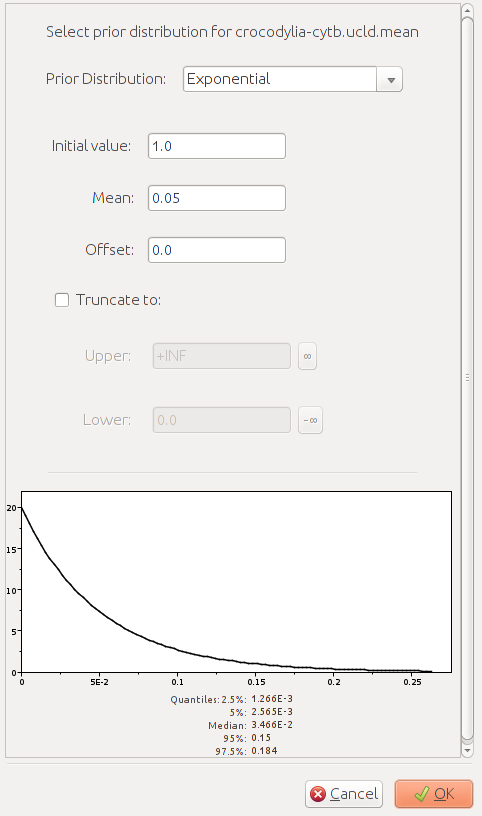
\includegraphics[width=\textwidth]{../screenshots/beauti-prior-ucldmean.jpg}
            \caption{crocodylia-cytb.ucld.mean.}
            \label{fig:beautiPriorsUcldMean}
        \end{subfigure}
        \begin{subfigure}[b]{0.29\textwidth}
            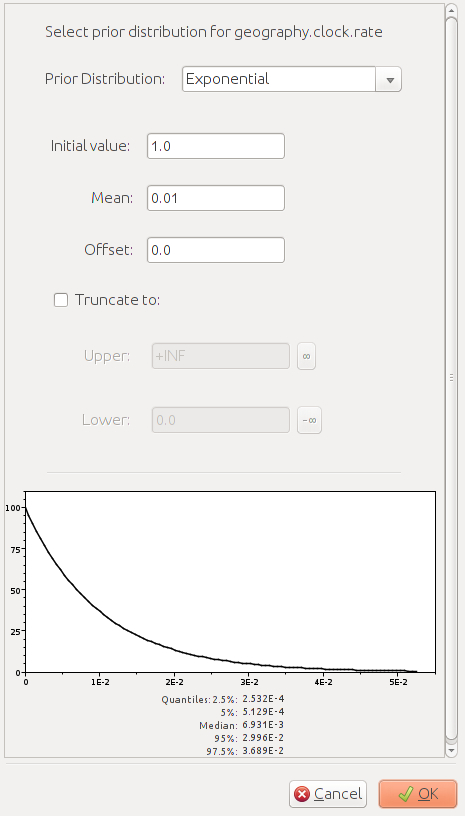
\includegraphics[width=\textwidth]{../screenshots/beauti-prior-clockrate.jpg}
            \caption{geography.clock.rate.}
            \label{fig:beautiPriorsClockRate}
        \end{subfigure}
        \begin{subfigure}[b]{0.31\textwidth}
            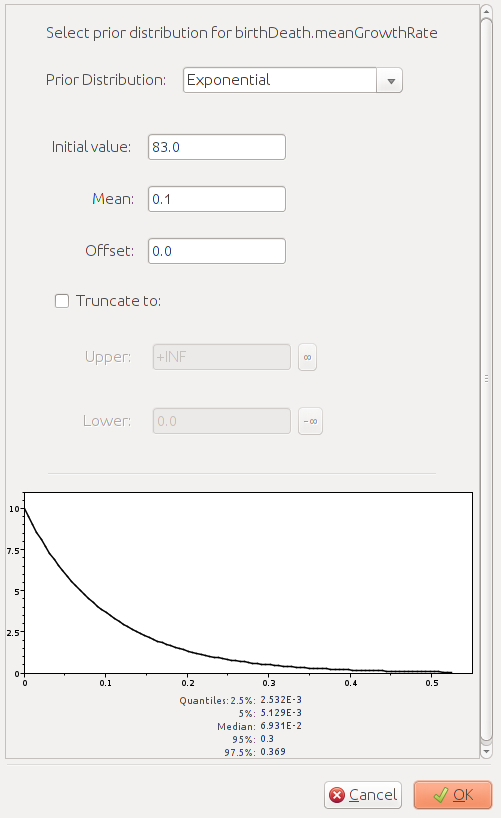
\includegraphics[width=\textwidth]{../screenshots/beauti-prior-birthrate.jpg}
            \caption{birthDeath.meanGrowthRate.}
            \label{fig:beautiPriorsBirthRate}
        \end{subfigure}
        \caption{Priors for clock rates and diversification rate.}
        \label{fig:beautiPriorsClocks}
    \end{figure}
}

\step{Select priors for node ages!}{
    Next, we need to specify our node-age priors based on fossil information.

    For \fieldvalue{tmrca(Alligatoridae)} select \fieldvalue{Gamma} for the
    \field{Prior Distribution}, and specify \fieldvalue{2} for both the
    \field{Shape} and \field{Scale} and \fieldvalue{64} for the
    \field{Offset}
    (Figure~\ref{fig:beautiPriorsAlligatoridae}).

    For \fieldvalue{tmrca(Crocodylus)} select \fieldvalue{Exponential} for the
    \field{Prior Distribution}, and specify \fieldvalue{10} for the mean
    and \fieldvalue{12} for the \field{Offset}
    (Figure~\ref{fig:beautiPriorsCrocodylus}).

    For \fieldvalue{tmrca(Caiman)} select \fieldvalue{Exponential} for the
    \field{Prior Distribution}, and specify \fieldvalue{4} for the mean
    and \fieldvalue{9} for the \field{Offset}
    (Figure~\ref{fig:beautiPriorsCaiman}).

    For \fieldvalue{treeModel.rootHeight} select \fieldvalue{Gamma} for the
    \field{Prior Distribution}, and specify \fieldvalue{78} for the
    \field{Initial value}, \fieldvalue{1.5} for the \field{Shape},
    \fieldvalue{6.0} for the \field{Scale}, and \fieldvalue{71.3} for the
    \field{Offset}. Also, make sure \field{Truncate to} is unchecked
    (Figure~\ref{fig:beautiPriorsRoot}).

    \begin{figure}[htbp]
        \centering
        \begin{subfigure}[b]{0.33\textwidth}
            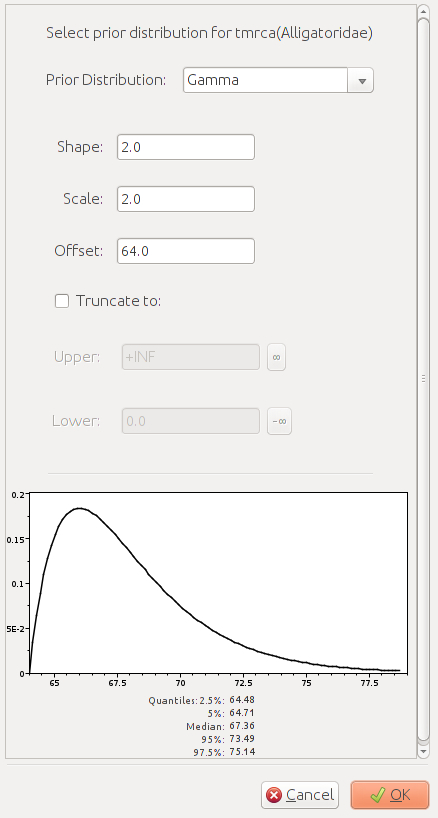
\includegraphics[width=\textwidth]{../screenshots/beauti-prior-alligatoridae.jpg}
            \caption{tmrca(Alligatoridae).}
            \label{fig:beautiPriorsAlligatoridae}
        \end{subfigure}
        \begin{subfigure}[b]{0.35\textwidth}
            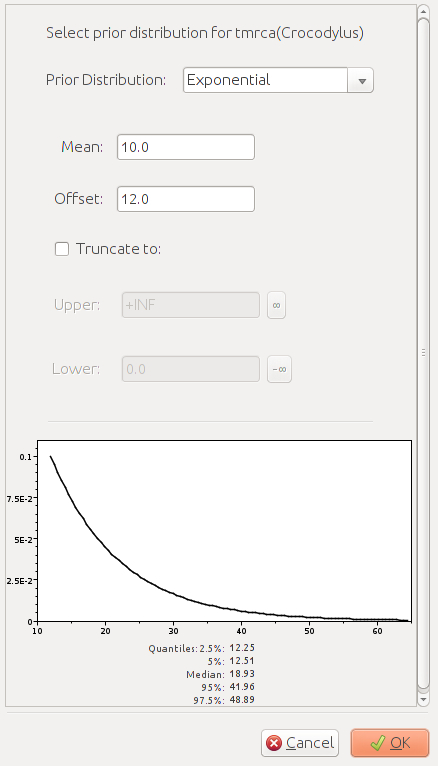
\includegraphics[width=\textwidth]{../screenshots/beauti-prior-crocodylus.jpg}
            \caption{tmrca(Crocodylus).}
            \label{fig:beautiPriorsCrocodylus}
        \end{subfigure}
        \begin{subfigure}[b]{0.35\textwidth}
            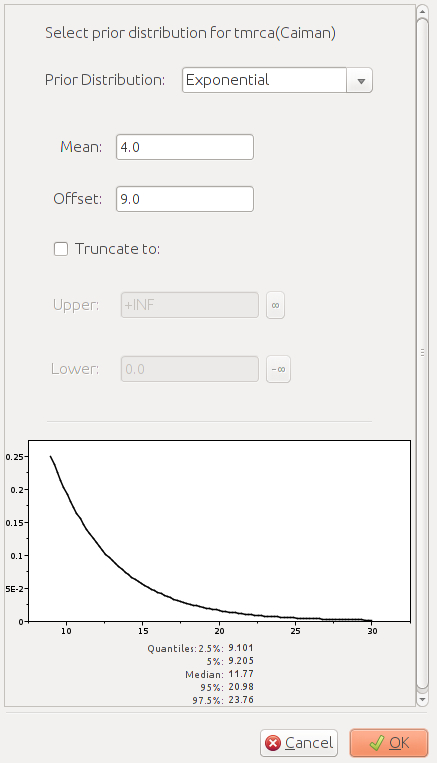
\includegraphics[width=\textwidth]{../screenshots/beauti-prior-caiman.jpg}
            \caption{tmrca(Caiman).}
            \label{fig:beautiPriorsCaiman}
        \end{subfigure}
        \begin{subfigure}[b]{0.315\textwidth}
            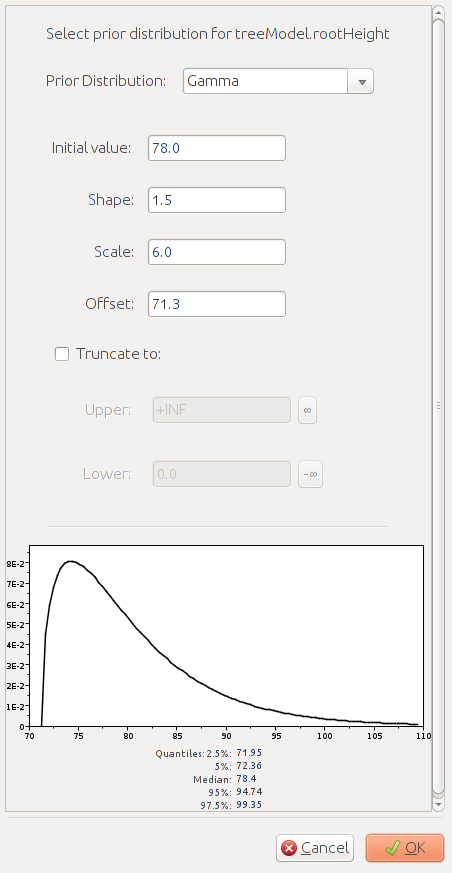
\includegraphics[width=\textwidth]{../screenshots/beauti-prior-root.jpg}
            \caption{treeModel.rootHeight.}
            \label{fig:beautiPriorsRoot}
        \end{subfigure}
        \caption{Priors for clock rates and diversification rate.}
        \label{fig:beautiPriorsClocks}
    \end{figure}
}


\newpage
\section{Additional Information/Resources}
Fantastic
\href{http://treethinkers.org/divergence-time-estimation-using-beast/}{tutorial}
and
\href{https://molevol.mbl.edu/wiki/images/6/6f/Bodega_2013_divtime_lecture.pdf}{slides}
by \href{http://phylo.bio.ku.edu/content/tracy-heath}{Tracy Heath}!

\newpage
\bibliography{../../bib/references}

\end{document}

